\documentclass{article}
\usepackage[margin=.75in]{geometry}
\usepackage{bookmark}
\usepackage{graphicx} % Required for inserting images
\usepackage{float}
\usepackage[titletoc,toc,page]{appendix}
\usepackage{wrapfig}
\usepackage{caption}
\usepackage{subcaption}
\usepackage{mathtools}
\usepackage{authblk}
\usepackage{hyperref}

\hypersetup{
    colorlinks,
    citecolor=blue,
    filecolor=blue,
    linkcolor=blue,
    urlcolor=blue
}

\floatstyle{plain} 
\restylefloat{figure}
\title{AST326 Lab 2: Introduction to Spectroscopy}
\author{Luke Wriglesworth \\ \small luke.wriglesworth@mail.utoronto.ca}
\date{\today}
\begin{document}
\maketitle

\begin{abstract}
  In this report, wavelength solutions are found for a one dimensional spectrum of an ideal blackbody, and for dispersed images of a supernova explosion, Jupiter, and The Moon. Data reduction techniques are applied to the dispersed images, and least squares fitting is used 
  to find a suitable model for the three sets of data. The wavelength solutions are used to find the temperature of the ideal blackbody, and to determine the velocity of a 1.644 micron Fe II emission visible in the dispersed image of the supernova. It will be shown that by 
  applying a linear least squares solution to the blackbody spectrum, its temperature can be calculated to be 4611.14 Kelvin, and by applying a quadratic polynomial fitting to the dispersed image of the supernova, its velocity can be determined to be 1293.1 km/s.
  Spectra of Jupiter and The Moon are obtained through a linear least squares fitting, and statistical analysis and error propagation techniques are applied to determine the validity of the three wavelength solutions and their resulting calculations. 
\end{abstract}


\section{Introduction}

Spectroscopy is a valuable tool for scientists of all disciplines, with it being especially important to astronomers. Spectroscopes split up light 
into its wavelength components, allowing astronomers to gain valuable information about distant targets, such as temperature, velocity, and the subject's molecular structure. 
Spectrometers obtain data using a CCD, which record photon intensity values at a given pixel position. To gain scientific information from this data, wavelength calibration must be performed, which is the process of finding a mathematical function that maps the pixel position of the CCD to the correct wavelength. One way of doing this is with a 
neon calibration lamp, since the spectral peaks of neon are well known. Another way is to use the near-infrared range OH emission lines in the atmosphere, which are also well known. 
The process for finding a wavelength solution from 1D and 2D sources will be outlined in this report using both of these techniques. 

These wavelength solutions will be applied to a spectrum of an unknown blackbody to determine its temperature, as well as a spectrum containing ionized
iron gas from a supernova explosion to determine the gas's velocity. Finally, a wavelength solution for the spectra of Jupiter and The Moon will be found 
from dispersed images obtained by the author's lab group.

Work for this experiment was done entirely independently among lab group members Tom Wu, Louis Branch, Yuqi Wang, and the author (Luke Wriglesworth). Only general conceptual information and our final results were exchanged between us after we obtained our data during the observatory session to 
determine if we were all on the right track. All the writing, code, plots, and conclusions in this report are the work of the author.  

\newpage

\section{Data and Observations}

\begin{wrapfigure}{r}{.30\textwidth}
  \vspace{-10pt}
  \caption{Dispersed image of ionized iron gas from a supernova explosion.}\label{wrap-fig:1}
  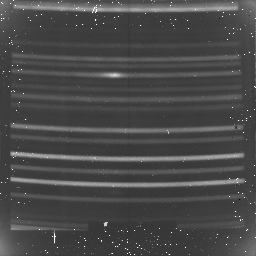
\includegraphics[width=.30\textwidth]{plots/near_infrared.png}
  \label{fig:near_infrared}
  \vspace{-10pt}
\end{wrapfigure} 

The data used in this experiment are obtained from three independent sources (summarized in Table \ref{tab:data_summary}), with the first two being provided by Professor Dae-Sik Moon. The first set of data is recorded using a USB4000 spectrometer. 
The device works by using a grating, which disperses photons before they are recorded onto a 1 dimensional detector in the form of numerical intensity values. The device is configured to be most 
sensitive to photons in the 500-800 nm range, and is equipped with a detector that records the intensity onto a 1024 pixel array. This spectrometer is used to obtain the spectrum of an unknown blackbody, 
which is displayed in Figure \ref{fig:bb_raw}. The goal with this set of data is to calculate the blackbody's temperature using its spectrum. To aid in calibrating the spectrometer, a spectrum of neon 
is used along with the known peaks of neon's spectrum (Figure \ref{fig:neon_raw}). The plots of the blackbody and the neon lamp spectrum used for calibration are shown together in Figure \ref{fig:part1_raw}.

The second set of data is a dispersed image containing ionized iron gas from a supernova explosion. It is obtained using a spectrograph with a 2D detector sensitive to the near-infrared range, meaning that
OH emission lines are present and easily identifiable in the background. A Fe II 1.644 micron emission is clearly visible in the upper third region of the image. The goal with this set of data is
to calculate the velocity of the Fe II emission. The dispersed image is shown in Figure \ref{fig:near_infrared}. 

The last set of data was obtained by our lab group on the rooftop of Burton Tower 
at the University of Toronto. We used a Meade LX200 10 inch telescope on a Sky Watcher CQ350 equatorial 
mount, equipped with a Shelyak Alpy spectrograph. The spectrograph has a resolution power $\approx \frac{1nm}{pixel}$ and covers the entire visible wavelength range. This device uses a grism, a combination of 
both a grating and prism to disperse the entering light into its components. During this observation session, dispersed images of The Moon (\ref{fig:moon_raw_fit}) and Jupiter (\ref{fig:jupiter_raw_fit}) were obtained and are shown in Figure \ref{fig:observations_raw}.

\begin{figure}[H]
  \centering
  \begin{subfigure}{.5\textwidth}
    \centering
    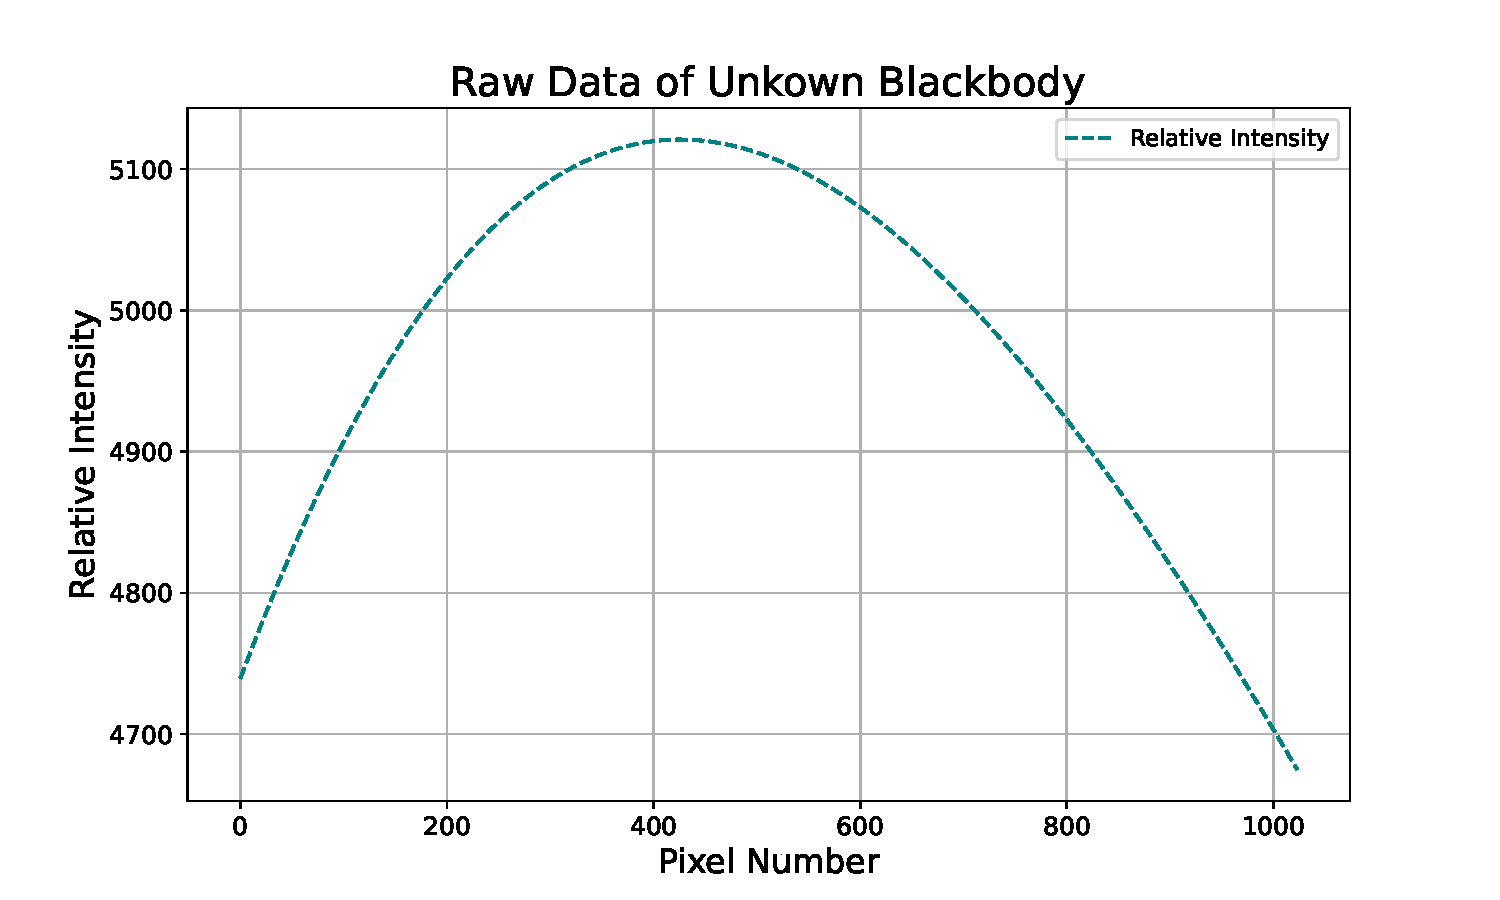
\includegraphics[width=\linewidth]{plots/raw_blackbody.pdf}
    \caption{Spectrum of the blackbody }
    \label{fig:bb_raw}
  \end{subfigure}%
  \begin{subfigure}{.5\textwidth}
    \centering
    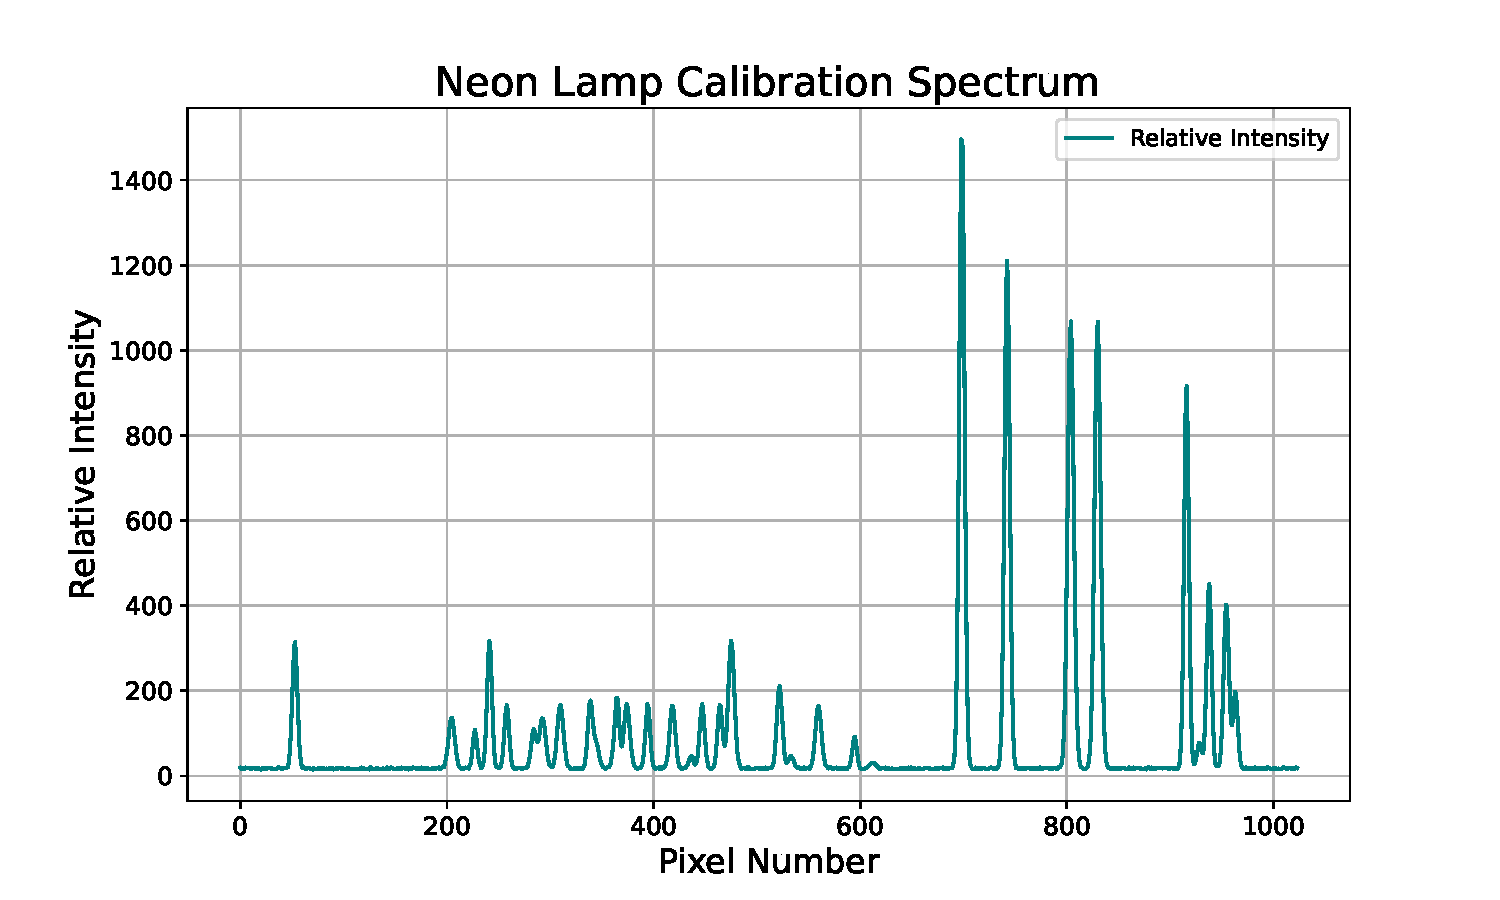
\includegraphics[width=\linewidth]{plots/neon_calibration_pt1.pdf}
    \caption{Neon spectrum used for calibration}
    \label{fig:neon_raw}
  \end{subfigure}
  \caption{Spectrum of the unknown blackbody, and the spectrum of a neon calibration lamp, both obtained using the same USB4000 spectrometer and plotted
  as a function of pixel position.}
\label{fig:part1_raw}
\end{figure}

\begin{figure}[h]
  \centering
  \begin{subfigure}{.3\textwidth}
    \centering
    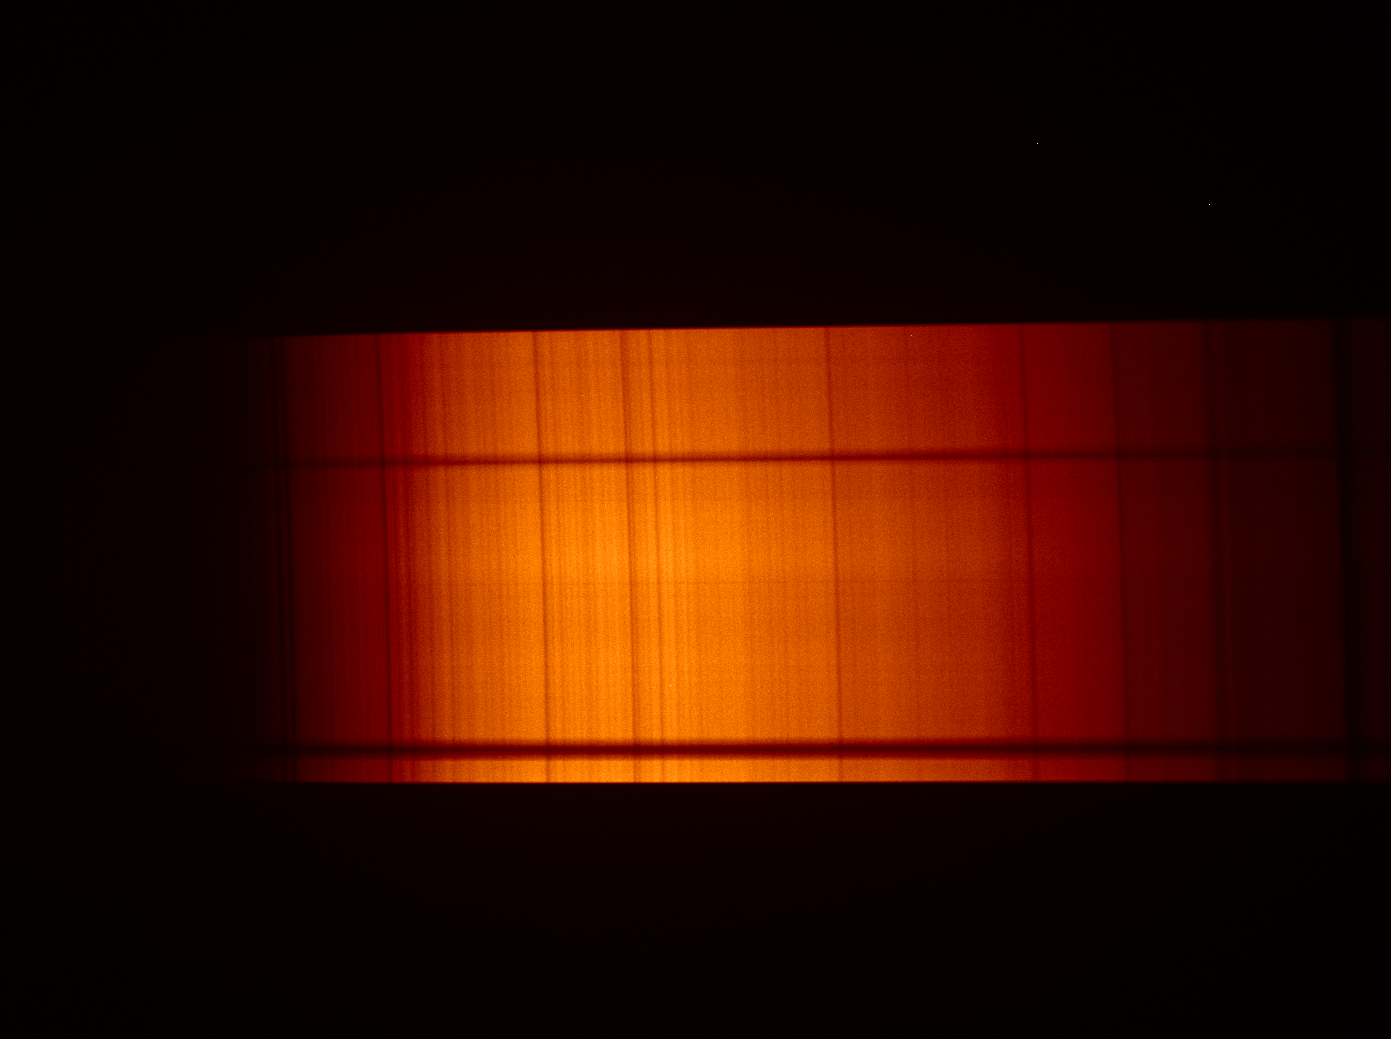
\includegraphics[width=\linewidth]{plots/moon_raw.png}
    \caption{The Moon}
    \label{fig:moon_raw_fit}
  \end{subfigure}%
  \begin{subfigure}{.3\textwidth}
    \centering
    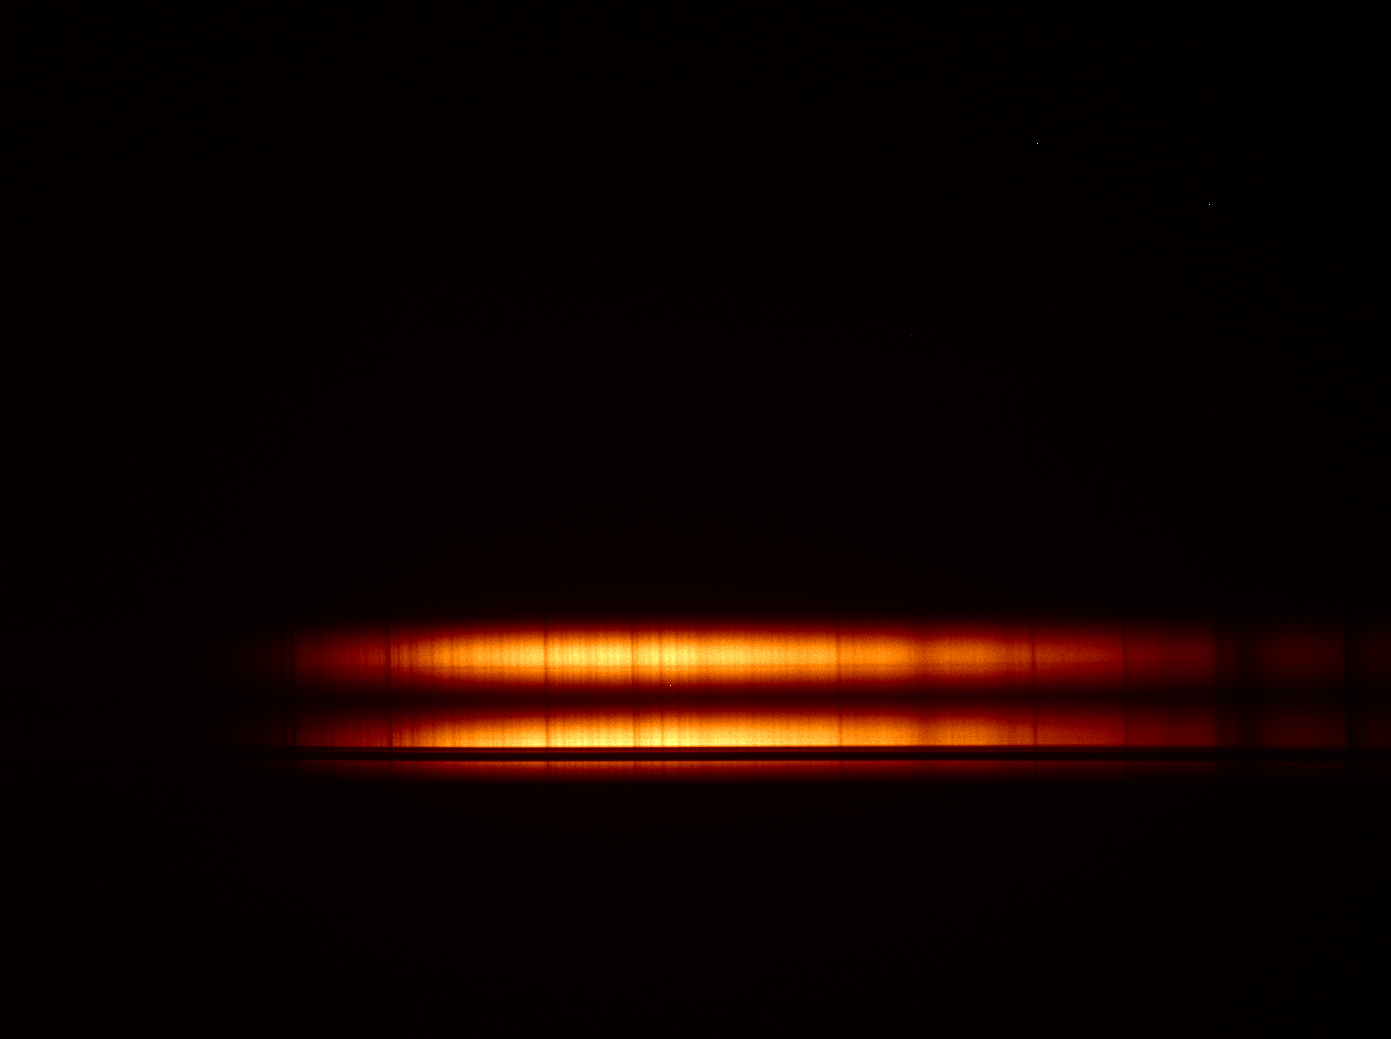
\includegraphics[width=\linewidth]{plots/jupiter_raw.png}
    \caption{Jupiter}
    \label{fig:jupiter_raw_fit}
  \end{subfigure}
  \caption{Dispersed images of The Moon, and Jupiter.}
\label{fig:observations_raw}
\end{figure}


\begin{table}[h]
  \centering
  \resizebox{\textwidth}{!}{%
  \begin{tabular}{|c|c|c|c|}
  \hline
   & \textbf{Data Set 1} & \textbf{Data Set 2} & \textbf{Data Set 3} \\
  \hline
  \textbf{Subject} & Unknown Blackbody  & Ionized iron gas from a supernova explosion & The Moon \& Jupiter\\
  \hline
  \textbf{Calibration Reference} & Neon Lamp Spectrum & OH Emission Lines & Neon Lamp Spectrum \\  
  \hline
  \textbf{Source} & Professor Dae-Sik Moon & Professor Dae-Sik Moon & Observed by the author\\
  \hline
  \textbf{Spectrometer} & Ocean Optics USB4000 & Unknown & Shelyak Alpy 600\\
  \hline
  \end{tabular}%
  }
  \caption{Summary of Relevant Data}
  \label{tab:data_summary}
\end{table}

\section{Data Reduction and Methods}

In terms of data reduction, there is not much work to be done with the first set of data, as 1D spectra of the blackbody and neon lamp have already been obtained.
For the second set of data, 1D spectra are extracted using DS9 over two rectangular regions differing only in their $x$ coordinates, which provide the median intensity of the region as a function of pixel position. 
This allows the two plots shown in Figure \ref{fig:OH_Spectrums} to be generated. The spectrum in Figure \ref{fig:isolated} is used for wavelength calibration using the known wavelengths
of the OH emission lines, and the spectrum in Figure \ref{fig:both} is used for further analysis of the Fe II emission.

\begin{figure}[H]
  \centering
  \begin{subfigure}{.5\textwidth}
    \centering
    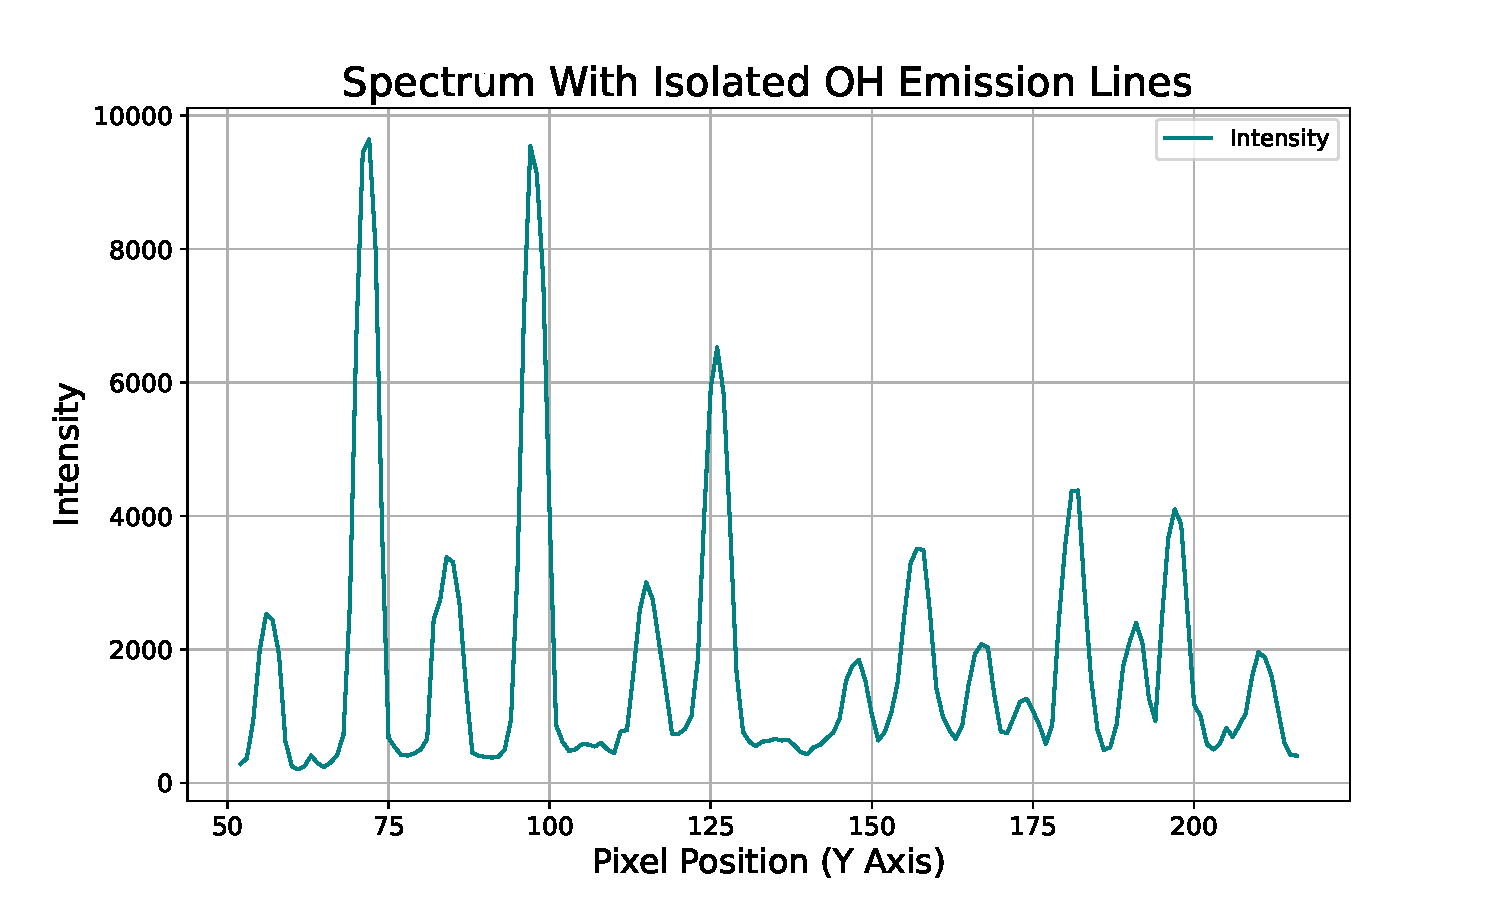
\includegraphics[width=\linewidth]{plots/OH_pixel_intensity.pdf}
    \caption{Isolated Spectrum of OH Emission Lines}
    \label{fig:isolated}
  \end{subfigure}%
  \begin{subfigure}{.5\textwidth}
    \centering
    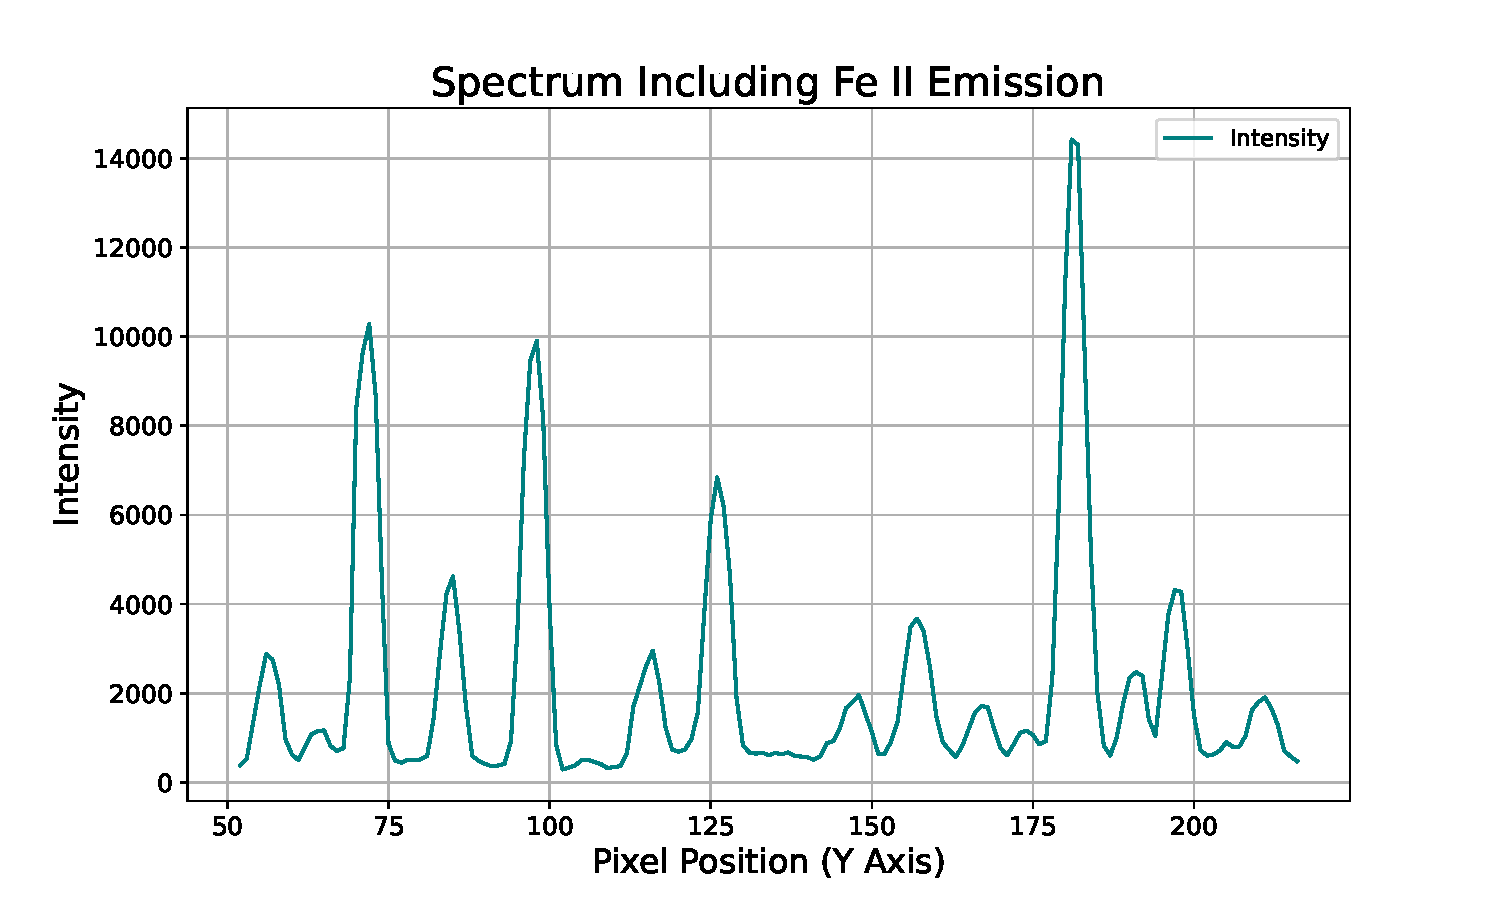
\includegraphics[width=\linewidth]{plots/supernova_pixels.pdf}
    \caption{Spectrum including ionized iron gas emission line}
    \label{fig:both}
  \end{subfigure}
  \caption{The two 1D spectra extracted from the 2D data. Spectrum (a) isolates only the OH emission lines, while 
  spectrum (b) also includes the Fe II emission}
\label{fig:OH_Spectrums}
\end{figure}

The data from our own observations requires the most amount of data reduction, as there are many sources of noise present in the images. Before 1D spectra can be extracted and analyzed, this noise must
be removed, or at least reduced as much as possible. First, not all parts of the detector in the spectrometer detect photons perfectly evenly. One part of the detector may have a higher baseline level of detection than another, 
so this must be corrected for. To combat this, a number of flat field images where the detector is uniformly illuminated are taken. Additionally, there is noise from the bias voltage required
to transfer electrons in the detector, as well as electrons generated by the detector itself that must be removed from the image. To account for this, a number of images with the detector isolated in a dark 
environment are taken. To produce the final image, the darks and flats are first median combined to make a master version of each, and then the final image is processed according to formula (\ref{eq:image}). The relevant Python code used for noise reduction
can be found in Appendix \ref{code:noise}.

\begin{equation}
  \label{eq:image}
  FinalImage = \frac{ScienceImage - MasterDark}{MasterFlat - MasterDark}
\end{equation}
\noindent
After the noise is reduced, the data is processed in the same manner as the second set of data. The extracted 1D spectra are displayed in Figure \ref{fig:1d_spectra}.

\begin{figure}[H]
  \centering
  \begin{subfigure}{.5\textwidth}
    \centering
    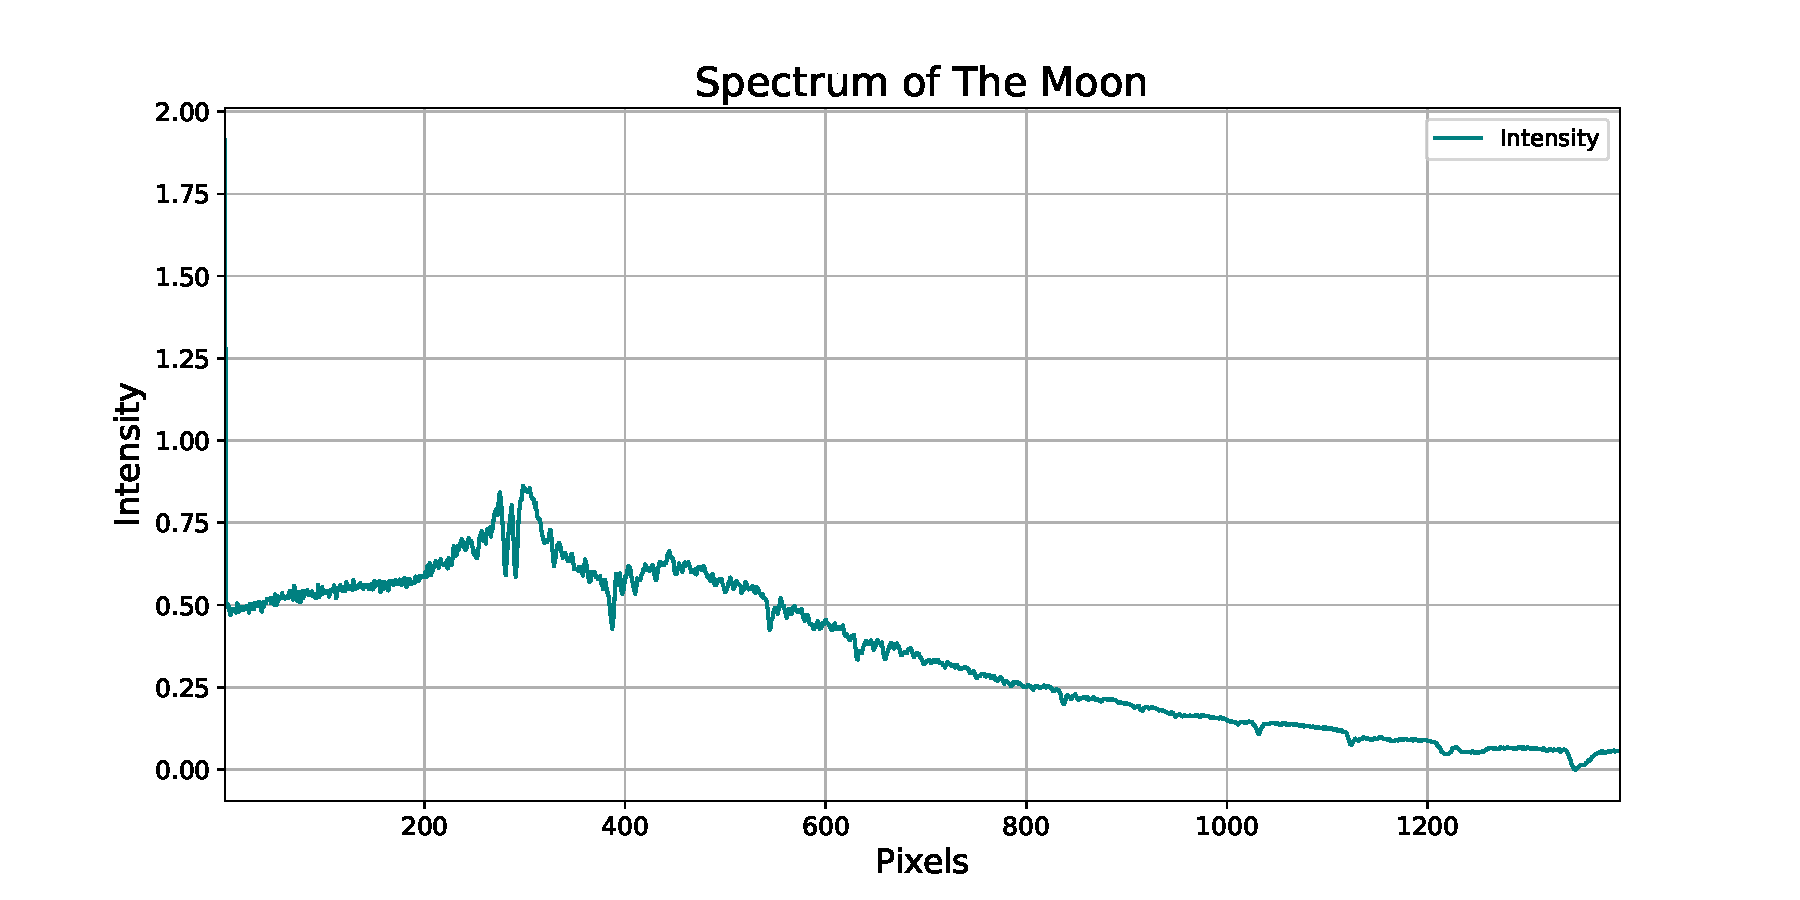
\includegraphics[width=\linewidth]{plots/obs_moon_pixels.pdf}
    \caption{1D spectrum of The Moon}
    \label{fig:moon_1D}
  \end{subfigure}%
  \begin{subfigure}{.5\textwidth}
    \centering
    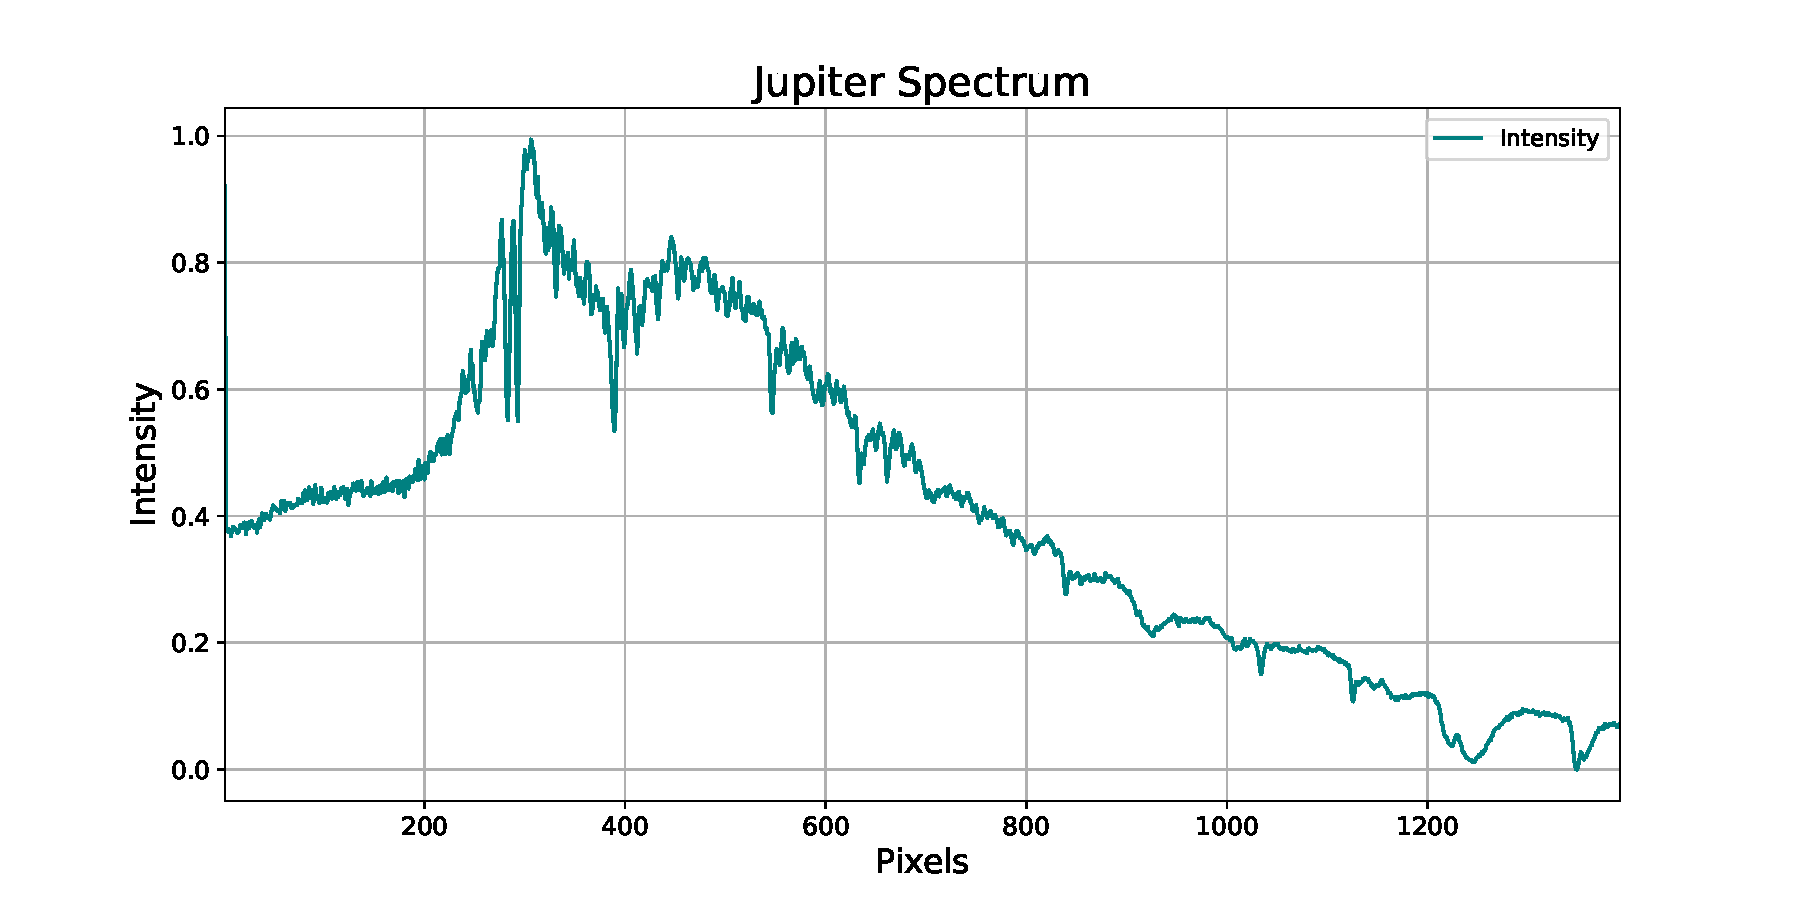
\includegraphics[width=\linewidth]{plots/obs_jupiter_pixels.pdf}
    \caption{1D spectrum of Jupiter}
    \label{fig:jupiter_1D}
  \end{subfigure}
  \caption{1D Spectra of The Moon (a) and Jupiter (b)}
\label{fig:1d_spectra}
\end{figure}

\section{Data Analysis and Modeling}

\subsection{Least Squares Fitting Background Information}

In order to get meaningful information from these plots, a wavelength solution must first be obtained, as the subject's intensity is currently only known 
as a function of pixel position. In other words, a function $f(x) = \lambda$ is needed, where $x$ is the pixel position in the spectral data and $\lambda$ is the true wavelength. One way 
to do this is to use the least squares method of polynomial fitting. First, we assume that the function $f(x)$ that relates pixel position and wavelength to be a polynomial of the form:

\begin{equation}
  \label{eq:1}
  f(x) = a_0 + a_1x + a_2x^2 + \ldots + a_nx^n
\end{equation}
And then insist on the additional condition that the sum of the squares of the residuals be minimized. In other words, we are minimizing the distance between $f(x)$ and the points in the spectrum that are known to correspond to specific wavelengths:
\begin{align*}
\frac{\partial}{\partial a_0} \sum_{i=1}^{m} [y_i - f(x_i)]^2 &= 0, \\
\frac{\partial}{\partial a_1} \sum_{i=1}^{m} [y_i - f(x_i)]^2 &= 0, \\
&\vdots \\
\frac{\partial}{\partial a_n} \sum_{i=1}^{m} [y_i - f(x_i)]^2 &= 0,
\end{align*}
\noindent
where $m$ is the number of data points, $y_i$ are the true wavelengths, and $f(x_i)$ are the predicted wavelengths given by the polynomial at pixel position $x_i$. 

\subsection{Peak Finding and Centroid Calculation}

\begin{table}[h]
  \centering
  \begin{tabular}{|c|c|c|c|}
  \hline
  \multicolumn{4}{|c|}{Identified Wavelengths (\AA)} \\
  \hline
  16128.608 & 16194.615 & 16235.376 & 16317.161 \\
  \hline
  16350.650 & 16442.155 & 16502.365 & 16553.814 \\
  \hline
  \end{tabular}
  \caption{Identified OH emission lines used for calibration}
  \label{tab:oh_lines_cal}
\end{table}


First, peaks in the OH emission spectrum that correspond to known wavelengths are picked out by hand (Table \ref{tab:oh_lines_cal}), and then their pixel positions are found using SciPy's \textit{find\textunderscore peaks()} function (Figure \ref{fig:oh_peaks}). 
The table of matched wavelengths for data sets 1 and 3 can be viewed in Appendix \ref{app:known_wavelengths}, and the plots of the identified peaks can be viewed in Appendix \ref{app:peaks}.

\begin{figure}[H]
  \centering
  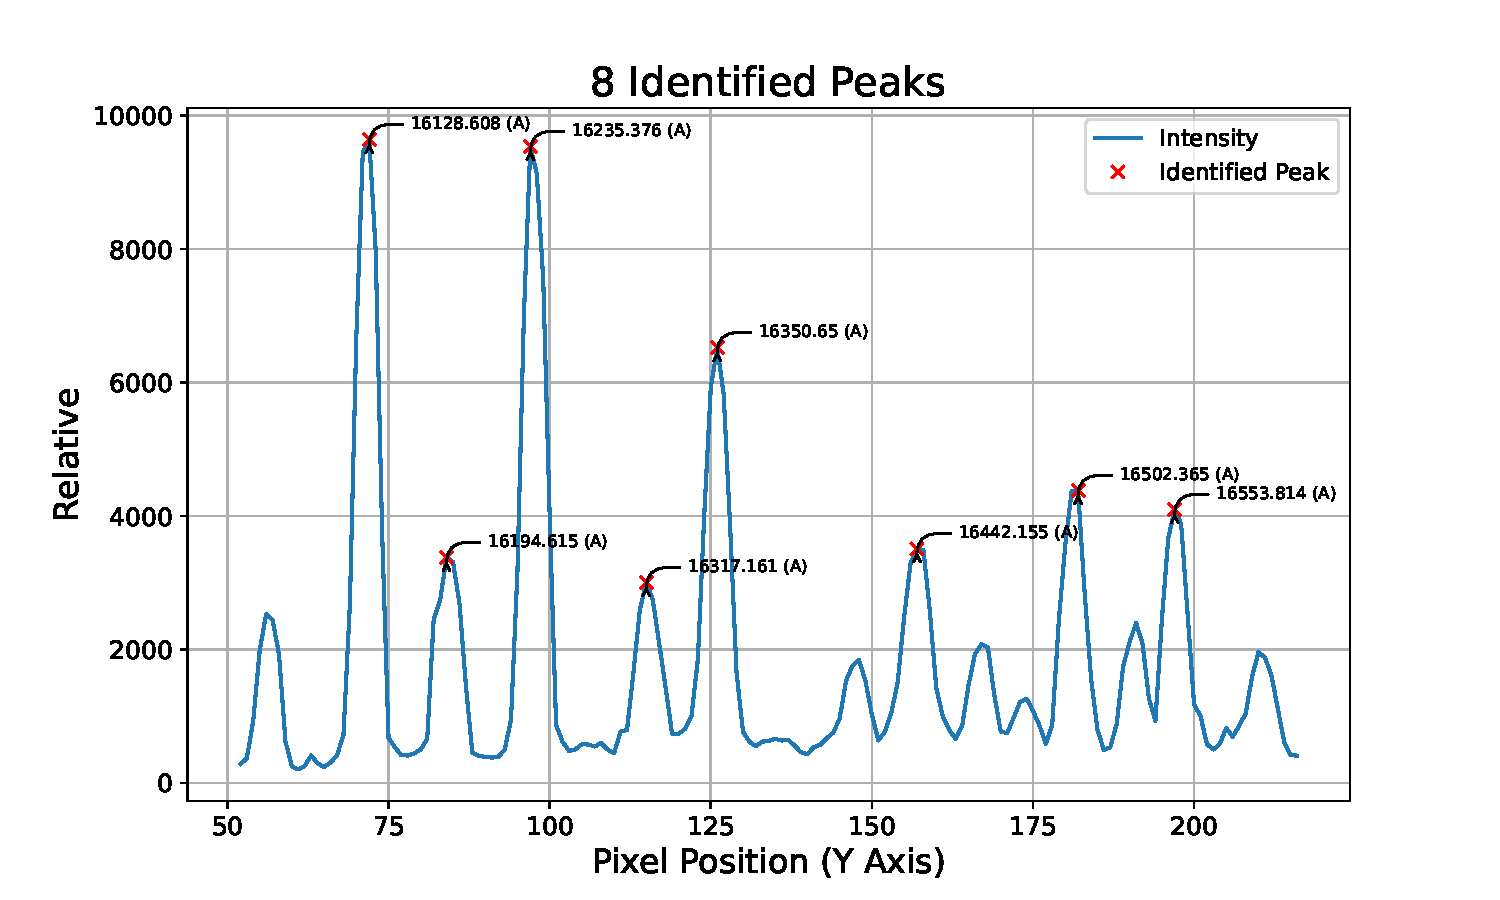
\includegraphics[width=.75\linewidth]{plots/OH_Peaks.pdf}
  \caption{Peaks in the spectrum that correspond to known OH emission lines}
  \label{fig:oh_peaks}
\end{figure}

As the peaks returned by \textit{find\textunderscore peaks()} are likely not completely accurate, the centroids of these peaks are calculated using the following formula, 
where $x_{cent}$ is the centroid's $x$ position, $x_i$ are the x values around the peak, and $I_i$ are the intensities at $x_i$:

\begin{equation}
  \label{eq:2}
  x_{cent} = \frac{\sum x_i I_i}{\sum I_i}
\end{equation}

\noindent
To use Formula \ref{eq:2}, appropriate values for $x_i$ need to be determined. This is done through trial and error, by trying to find a
symmetrical boundary around the peak that encloses it without overlapping into the neighbouring peaks. An example of this process can be seen being applied to the 
OH emission lines in Figure \ref{fig:oh_boundary}. The plots for the other two data sets can be viewed in Appendix \ref{app:centroid_bounds}. 

\begin{figure}[H]
  \centering
  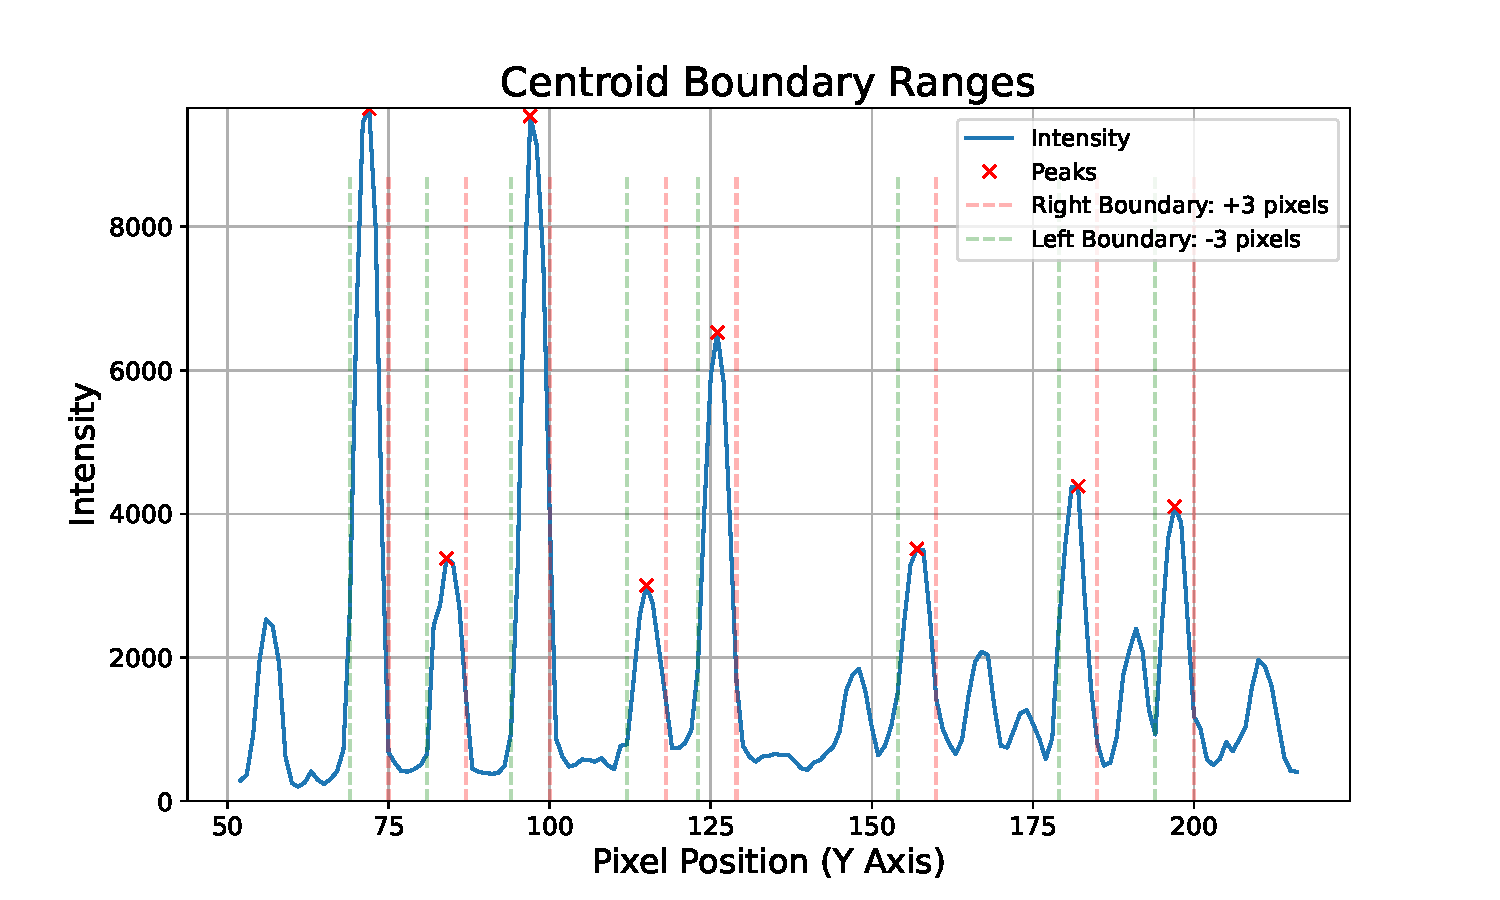
\includegraphics[width=.7\linewidth]{plots/OH_Centroid_Boundaries.pdf}
  \caption{Centroid boundary ranges for the OH emission lines}
  \label{fig:oh_boundary}
\end{figure}

\noindent
Next the centroids can be calculated using Equation \ref{eq:2} (Figure \ref{fig:centroids_oh}). The relevant Python code for peak and centroid finding can be viewed in Appendix \ref{code:centroids}.

\begin{figure}[H]
  \centering
  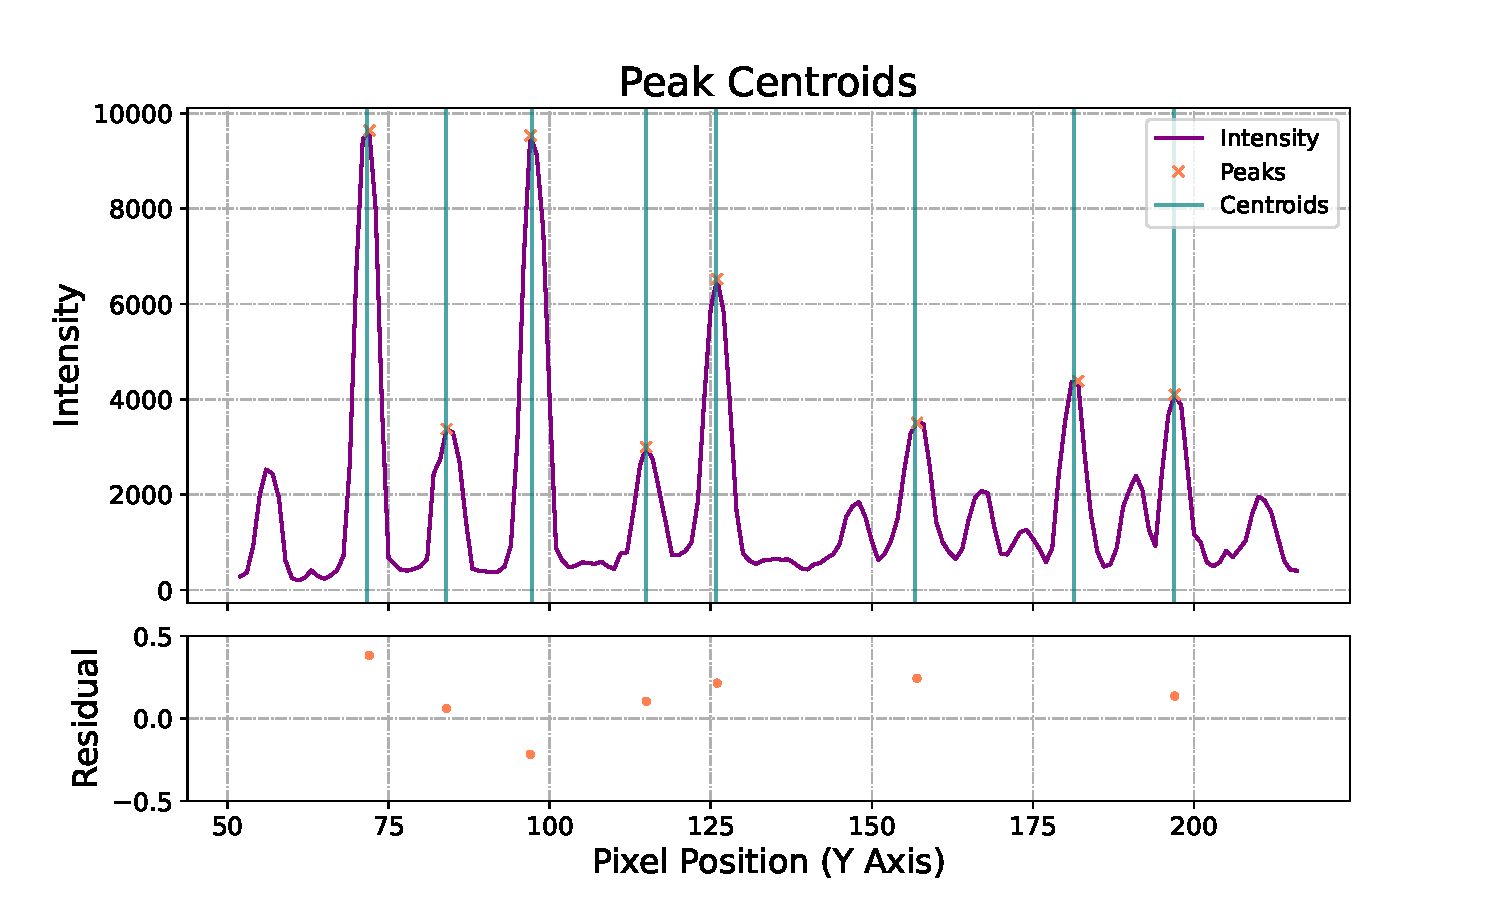
\includegraphics[width=.7\linewidth]{plots/OH_Centroids_Residuals.pdf}
  \caption{Centroids calculated for the OH emission peaks and their residuals}
  \label{fig:centroids_oh}
\end{figure}

\subsection{Wavelength Solution}
Now the wavelength solution for the OH emission line spectrum can be found. Using NumPy's \textit{polyval()} function with polynomial degrees 1, 2, and 3, the solutions shown
in Figure \ref{fig:oh_solutions} are generated.

\begin{figure}[H]
  \centering
  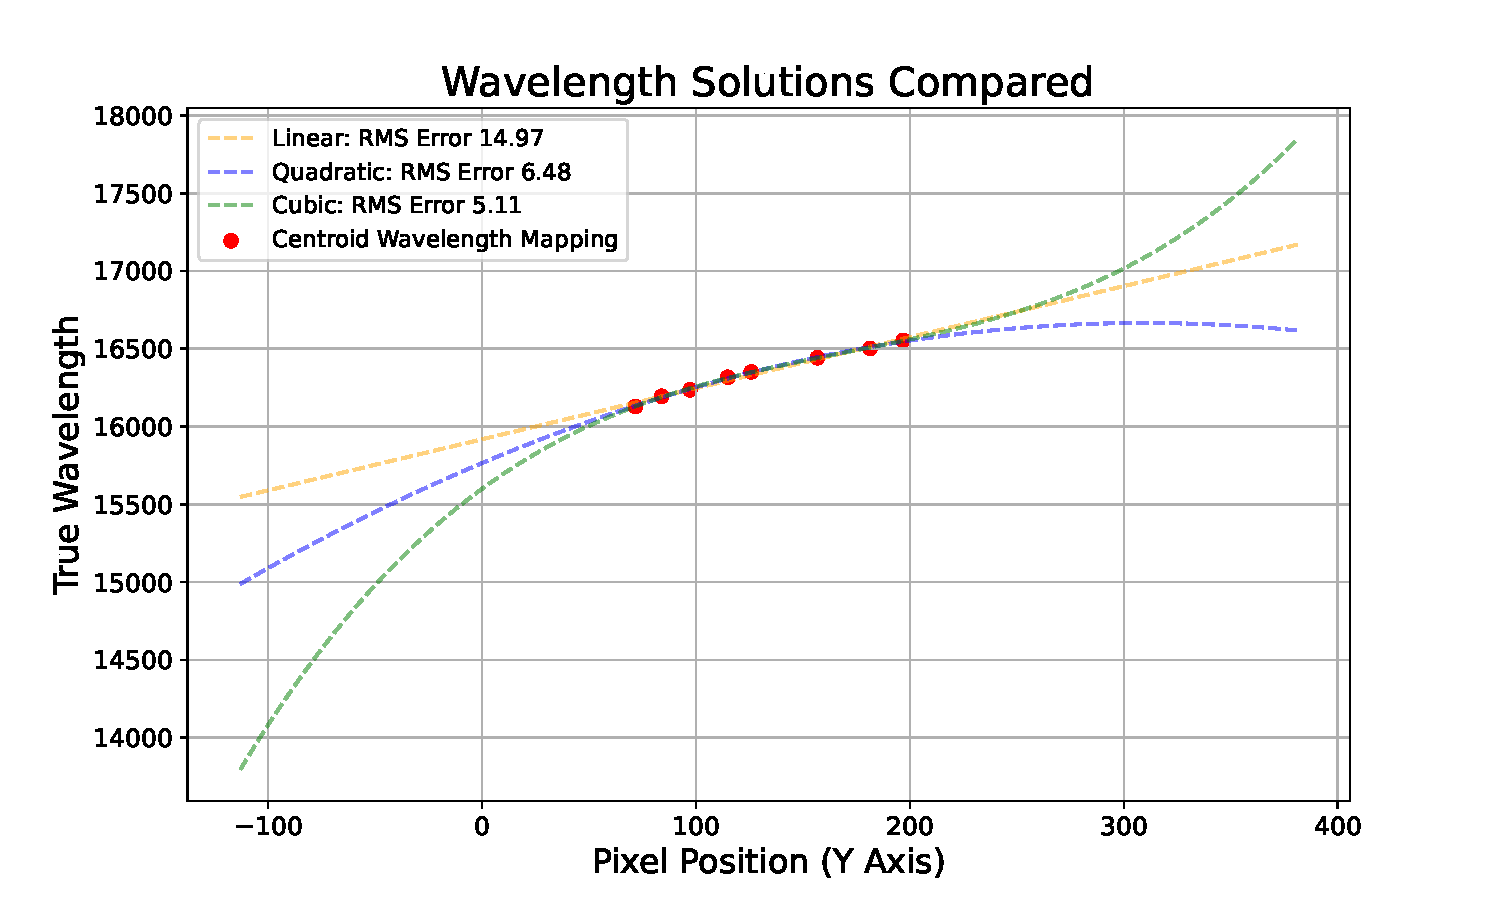
\includegraphics[width=.85\linewidth]{plots/OH_Sol_Comparison.pdf}
  \caption{Possible wavelength solutions for the OH emission lines}
  \label{fig:oh_solutions}
\end{figure}

\begin{figure}[H]
  \centering
  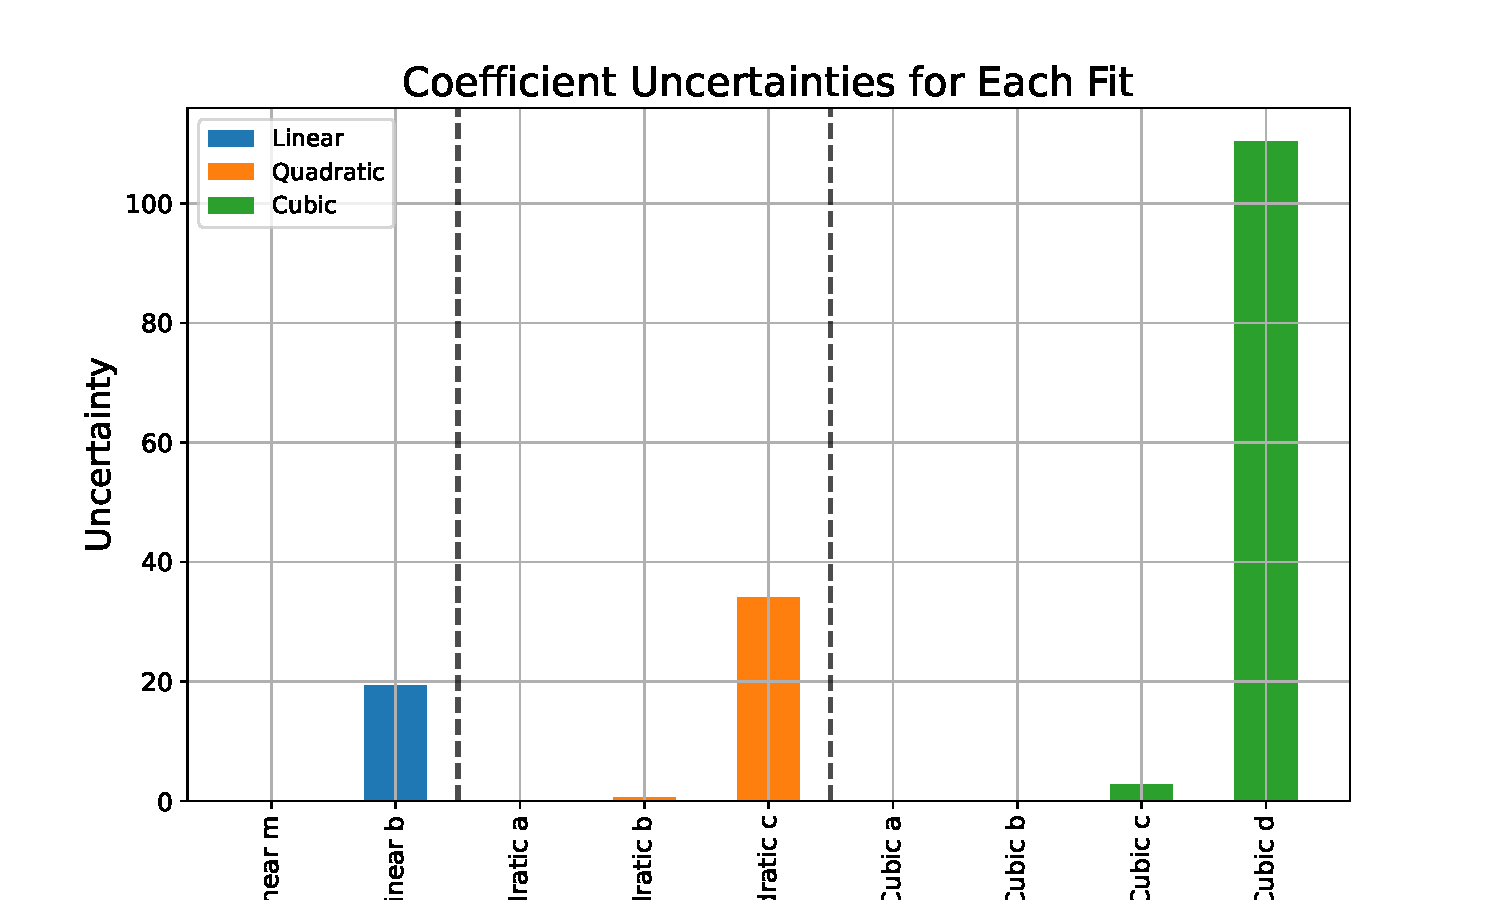
\includegraphics[width=.7\linewidth]{plots/OH_Coef_Uncerctainty.pdf}
  \caption{Uncertainties of the coefficients for each solution, calculated from the square root of the diagonals of the covariant matrix}
  \label{fig:oh_coef}
\end{figure}

With so few known wavelengths to go by, it is tough to determine the proper fit that generalizes the distribution without overfitting. As shown in Figure \ref{fig:oh_solutions}, 
the linear solution best generalizes the data over a very large range of pixels, but since calculations will be done around the 180 pixel region specifically and not far out from the sample point range, it makes sense to be more precise with the solution. The residuals for each solution are shown in Figure \ref{fig:oh_res}, with the quadratic and cubic residuals sharing
the same underlying pattern, indicating that higher degree solutions are fitting only underlying noise in the data and should be avoided. Additionally, the root-mean-square error of the quadratic residuals are only larger than the cubic solution by a factor
of around 1.27, as shown in Figure \ref{fig:oh_solutions}. Therefore, choosing the cubic polynomial will not significantly reduce the RMS error. In Figure \ref{fig:oh_coef}, the uncertainties of each of the coefficients of the polynomials are displayed, calculated from the square roots of the covariant matrix diagonals. A large jump in uncertainty is observed
with the cubic polynomial without a proportional decrease in RMS error in the residuals. For these reasons, the quadratic solution is the best choice as it fits each of the data points very well while still providing a more general fitting of the data than the cubic solution.  

By following the same set of logic, solutions for the USB4000 and Shelyak Alpy spectrometer data sets are also determined. Both of them can best be modelled as a linear distribution. 
The analogues of Figures \ref{fig:oh_solutions}, \ref{fig:oh_coef}, \ref{fig:oh_quad}, and \ref{fig:oh_res} for the other two spectrometers can be viewed in Appendix \ref{app:solutions}.

\begin{figure}[H]
  \centering
  \begin{subfigure}{.65\textwidth}
    \centering
    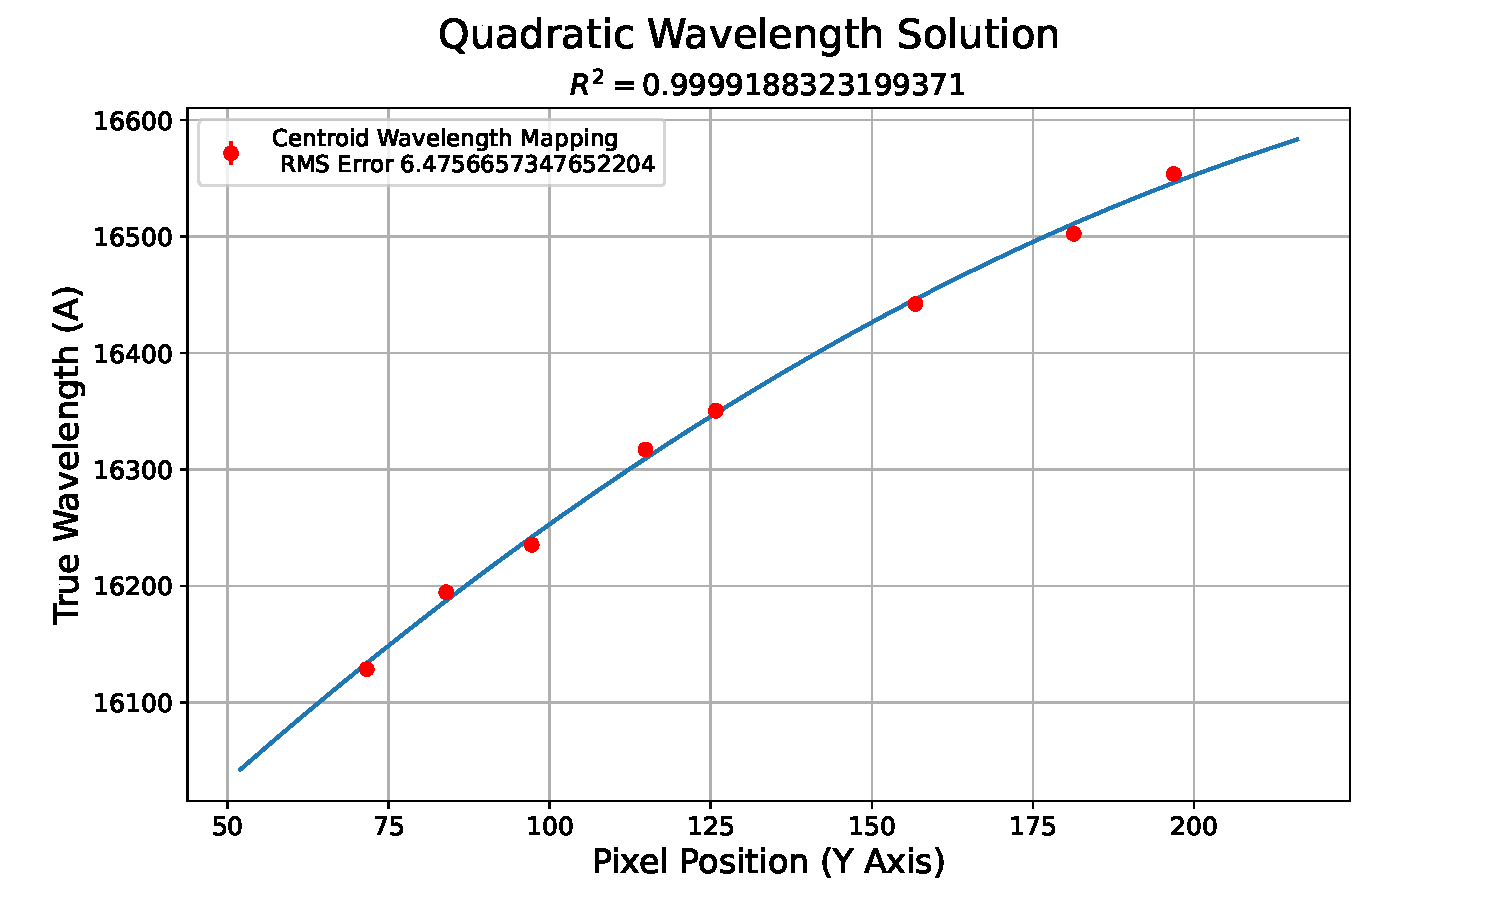
\includegraphics[width=\linewidth]{plots/OH_Quadratic.pdf}
    \caption{Quadratic wavelength solution for the OH emission lines}
  \end{subfigure}%
  \begin{subfigure}{.30\textwidth}
    \centering
    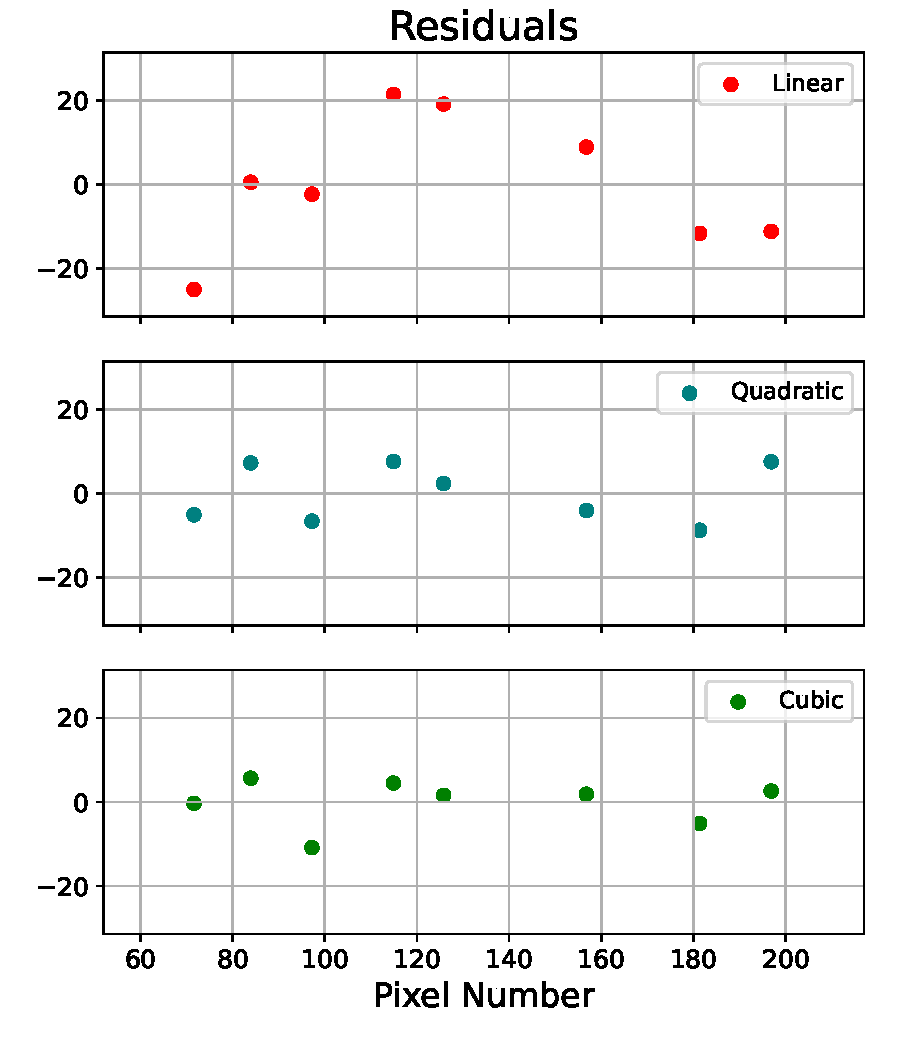
\includegraphics[width=\linewidth]{plots/OH_Sol_Residuals.pdf}
    \caption{Solution residuals for each polynomial degree}
    \label{fig:oh_res}
  \end{subfigure}
  \caption{Plot of the quadratic wavelength solution applied to the OH emission lines and the residuals}
  \label{fig:oh_quad}
\end{figure}


\section{Discussion}

\subsection*{Blackbody Temperature}

Now that wavelength solutions are known for each data set, they are used as tools for finding additional information about the measurement subjects. In the case of the blackbody measured using the USB4000 spectrometer,
its peak wavelength can now be found and used to determine the blackbody's temperature. The blackbody's wavelength solution can be seen in Figure \ref{fig:bb_solution} applied to the spectrum, and its peak wavelength was determined to be $\approx$ 628.4285223741275 nm. Using 
this information we can calculate the blackbody's temperature using Wien's Law (Equation \ref{eq:wien}), where $T$ is the object's temperature at wavelength $\lambda_{peak}$ and $b$ is a constant of proportionality $\approx 2.897771955 \times 10^{-3} m \ K$.
The Python code for these calculations can be found in Appendix \ref{code:temperature}.

\begin{figure}[H]
  \centering
  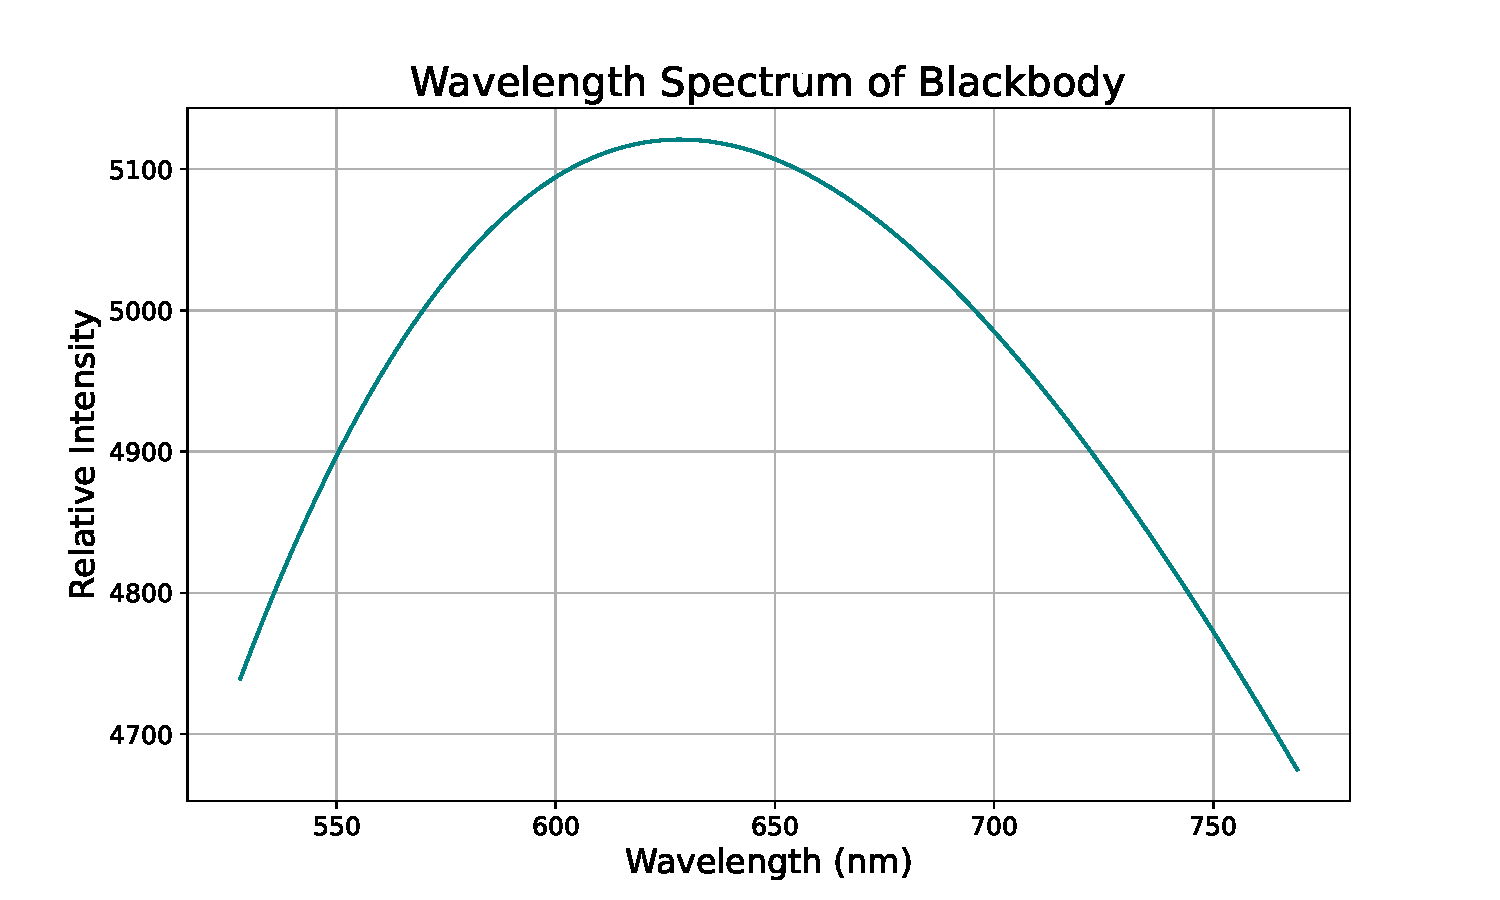
\includegraphics[width=.7\linewidth]{plots/blackbody_solution.pdf}
  \caption{Linear wavelength solution applied to the blackbody}
  \label{fig:bb_solution}
\end{figure}

\begin{equation}
  \label{eq:wien}
  T = \frac{b}{\lambda_{peak}} \\
\end{equation}

\begin{equation}
  T \approx \frac{2.897771955 \times 10^-3}{628.4285223741275 \times 10^{-9}}\frac{m \ K}{m}
\end{equation}

\begin{equation}
  T \approx 4611.140092834369 K \approx 4611.14 K
\end{equation}

\subsection{Fe II Emission Velocity}

By applying the wavelength solution to the spectrum containing the Fe II emission, we are able to use Doppler shift 
to find the emission's velocity. Formula (\ref{eq:doppler}) will be used, where $\lambda_{obs}$ is the observed wavelength of the light, $\lambda_i$ is the intrinsic
wavelength of the light, $c$ is the speed of light in $\frac{m}{s}$, and $v$ is the velocity of the object emitting the light relative to the observer.

\begin{equation}
  \label{eq:doppler}
  v = c\frac{\lambda_{obs} - \lambda_i}{\lambda_i}
\end{equation}

\begin{figure}[H]
  \centering
  \includegraphics*[width=.7\linewidth]{plots/supernova_centroid.pdf}
  \caption{Pixel position of the Fe II emission}
  \label{fig:supernova_pixel}
\end{figure}

The centroid pixel position of the Fe II emission was found to be at pixel location 181.23 (Figure \ref{fig:supernova_pixel}), which the quadratic wavelength solution maps to a peak wavelength of $16510.8916965 \ \AA$. It is also known that Fe II has an 
intrinsic wavelength of $1.6439981 \ \mu m$, or $1.6439981 \times 10^4 \ \AA$. These two values are enough to calculate the Fe II emission's velocity using Equation \ref{eq:doppler}:

\begin{displaymath}
  v = c\frac{(16510.8916965 - 1.6439981 \times 10^4)}{1.6439981} \frac{m \ \AA}{s \ \AA} = 1293.0971168075641 \ m/s \approx 1293.1 \ km/s
\end{displaymath}

\subsection{Wavelength Solutions of Jupiter and The Moon}

\begin{figure}[H]
  \centering
  \begin{subfigure}{.5\textwidth}
    \centering
    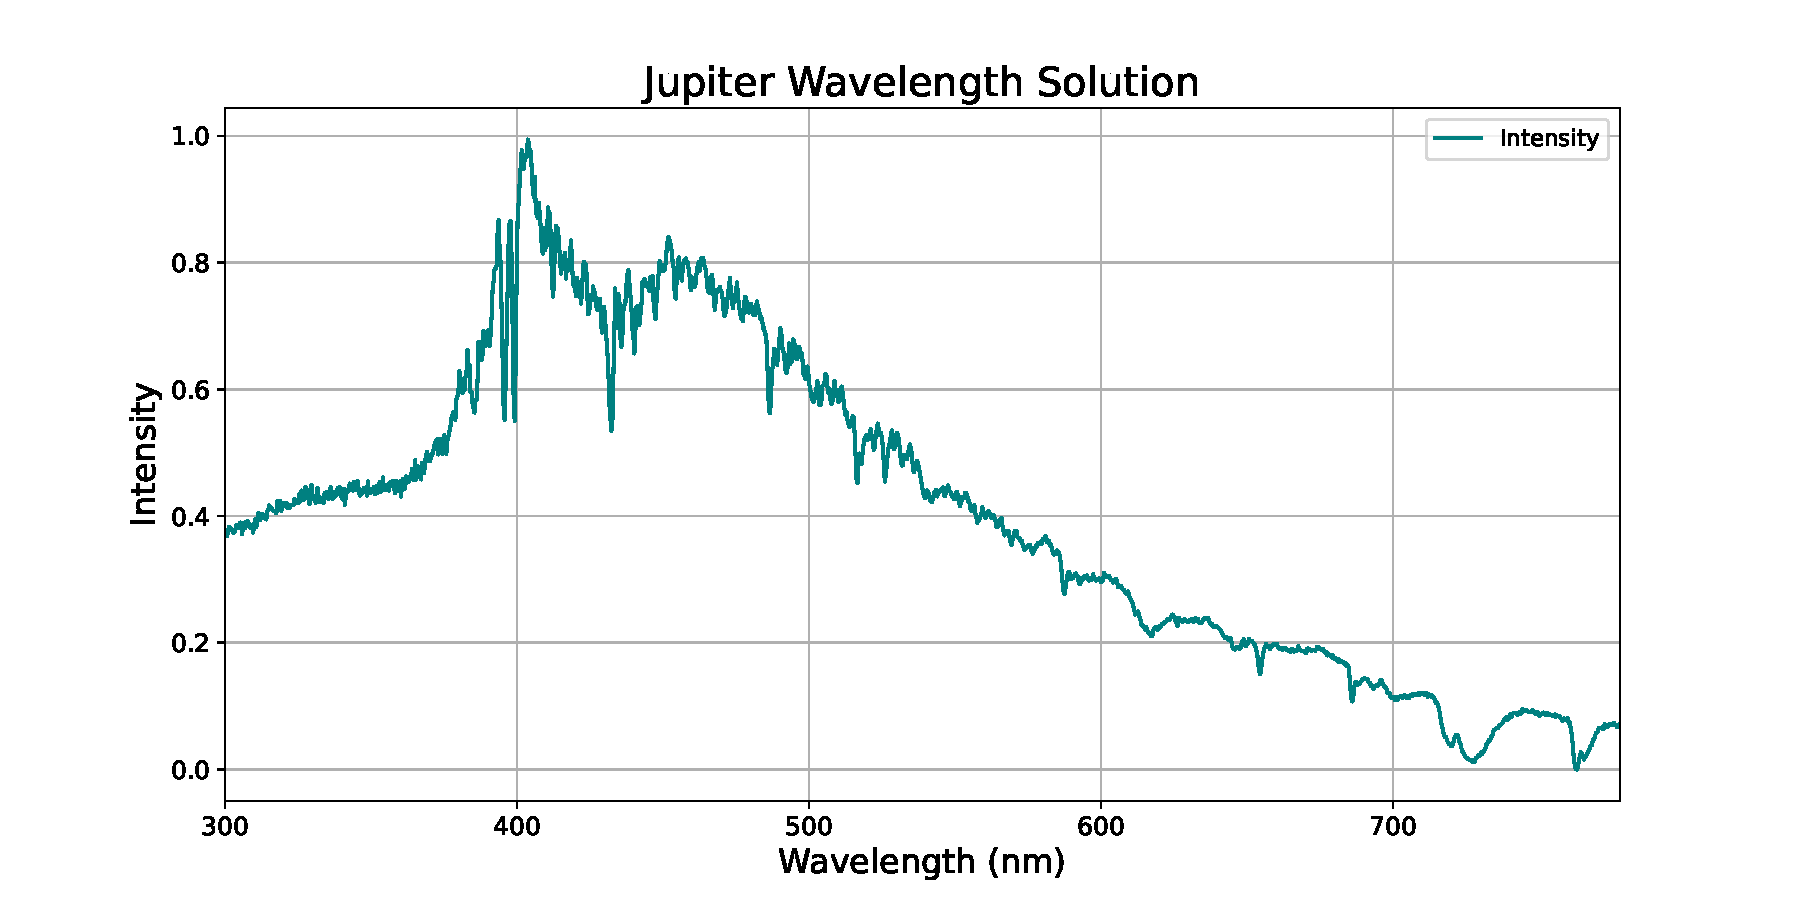
\includegraphics[width=\linewidth]{plots/obs_jupiter_spectrum.pdf}
    \caption{Spectrum of Jupiter}
    \label{fig:jup_wav}
  \end{subfigure}%
  \begin{subfigure}{.5\textwidth}
    \centering
    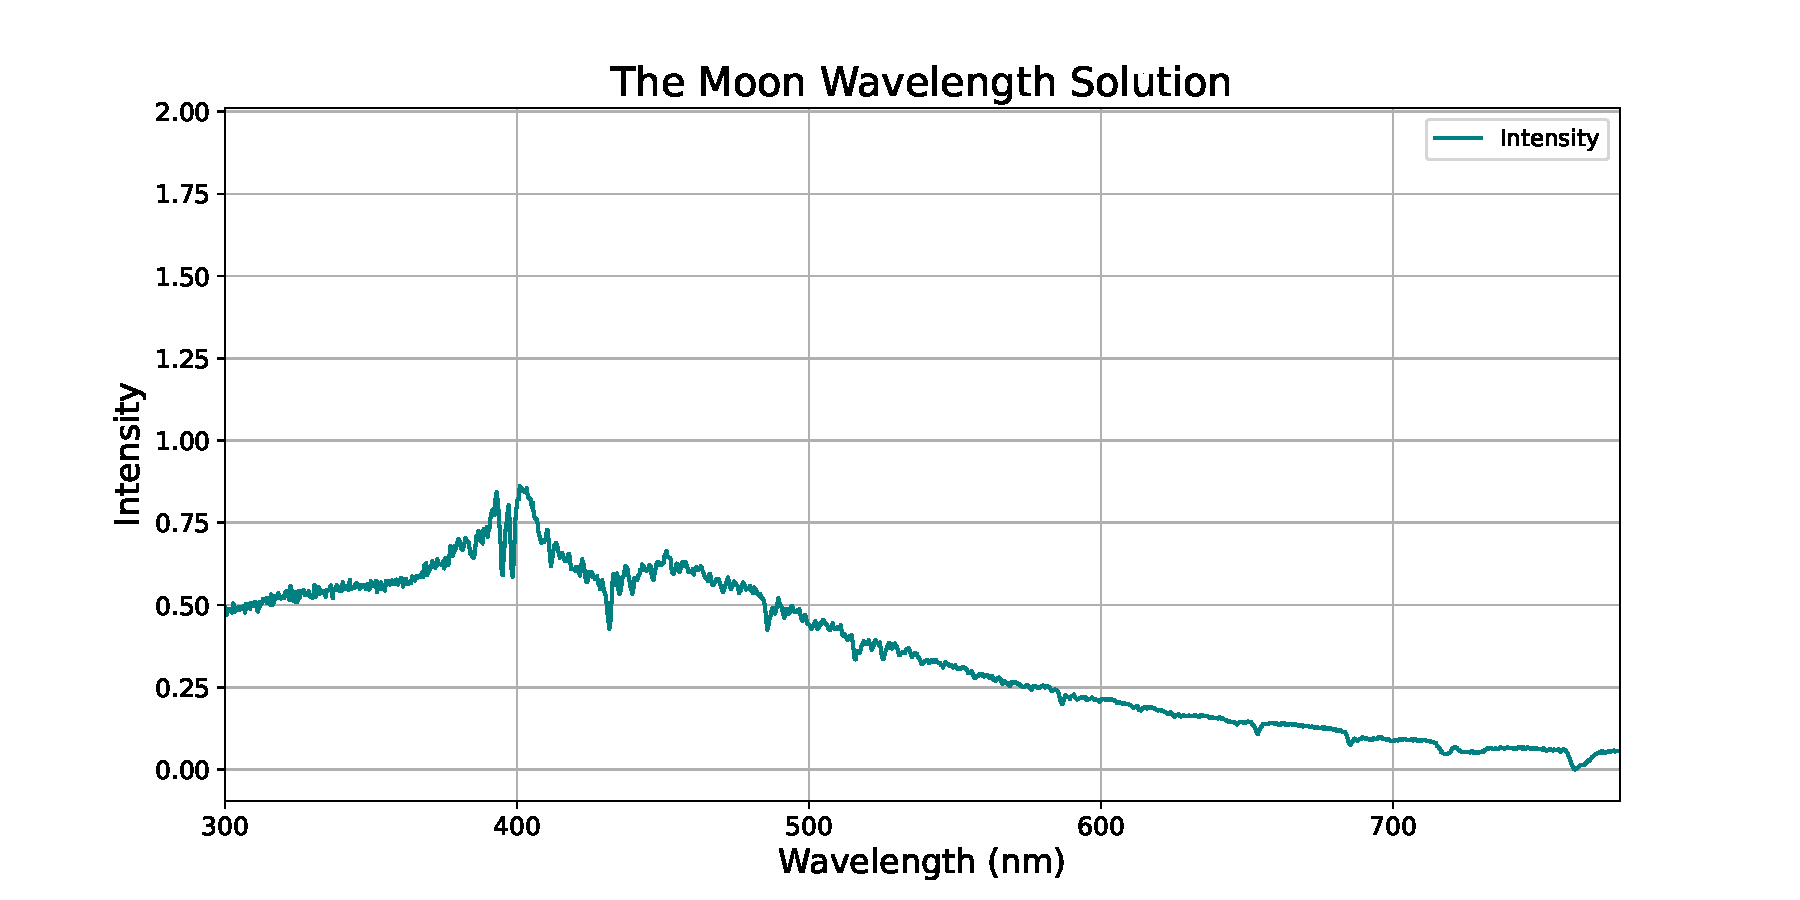
\includegraphics[width=\linewidth]{plots/obs_moon_spectrum.pdf}
    \caption{Spectrum of The Moon}
    \label{fig:moon_wav}
  \end{subfigure}
  \caption{Linear wavelength solutions applied to Jupiter (a), and The Moon (b)}
\label{fig:obs_spectrums}
\end{figure}

By applying the linear wavelength solution found for the Shelyak Alpy spectrometer, spectra of Jupiter (Figure \ref{fig:jup_wav}) and The Moon (Figure \ref{fig:moon_wav}) are found.
It is unsurprising that both of these spectrums have peaks in the same location, at around 400 nm. The dispersed light that makes up each spectrum is really from a single source, The Sun. Although the sun 
typically peaks at around 500 nm in the visible spectrum, the 100 nm shift seen in Figures \ref{fig:jup_wav} and \ref{fig:moon_wav} may be the result of the scattering of light when it passes through 
Earth's atmosphere.

\subsection{Error Analysis}
In the first set of data, there are two main sources of error that influence the results of the experiment. The first source of error comes from the placement of the centroids
in the wavelength solution, as this can vary based on the parameters given to the \textit{find\textunderscore peaks()} function. The second source comes from the polynomial fitting itself. In order to quantify this, the following 
standard error propagation formula is used:

\begin{equation}
  s_f = \sqrt{(\frac{\partial f}{\partial x})^2 s_x + (\frac{\partial f}{\partial y})^2 s_y + (\frac{\partial f}{\partial z})^2 s_z + \dots}
\end{equation} 


Here, $s_f$ is the final RMS error in the answer, and $s_x$, $s_y$, and $s_z$, are the RMS errors in each of the individual calculations. $f$ is taken to be the function representing the final calculation in the program, and each partial derivative to represent the change in $f$ with respect to the 
independent variables $x$, $y$, and $z$, which are the sources of error. For example, in the centroid placement for the initial wavelength calibration in data set 1, it was determined by running the full program many times that the final temperature changes by approximately 1.73 Kelvin for each 
change in pixel position around the initial centroid placement. Thus,  

\begin{equation}
  \frac{\partial f}{\partial x} \approx \frac{1.73}{1 pixel}
\end{equation}

\noindent
For the calculations regarding the polynomial fitting, $\frac{\partial f}{\partial y}$ is taken to be the analytic derivative of the polynomial evaluated at the pixel position of the 
relevant calculation, with $s_y$ being the RMS error of the solution's residuals. A summary of all the relevant data used for the error propagation is shown in Table \ref{tab:q1_errors}, and the 
Python code for these calculations can be viewed in Appendix \ref{code:error}.

\begin{table}[h]
  \centering
  \begin{tabular}{|c|c|}
  \hline
  Initial centroid placement RMS Error &  0.31 \\ \hline
  $\frac{\partial f}{\partial x}$ for initial centroid placement & 1.73 \\ \hline
  Linear solution RMS error in residuals & 0.88 \\ \hline
  $\frac{\partial f(x_{peak})}{\partial y}$ for linear solution & 0.24 \\ \hline
  \end{tabular}
  \caption{Summary of the relevant variables for error propagation in the USB4000 spectrometer data set}
  \label{tab:q1_errors}
\end{table}

\noindent
Now an estimate of the final RMS error is calculated:

\begin{equation}
  s_f \approx \sqrt{(\frac{1.73 \ K}{pixel})^2(0.31) + (\frac{0.24 \ K}{pixel})^2(0.88)} \approx 0.98 \ K
\end{equation}

\noindent
Therefore, the RMS error on the final temperature is around 1 Kelvin. In the case of the velocity calculations for the Fe II emission, the peak centroid calculation for the emission must also be included as a third variable in the error propagation formula. All the relevant data used
for the calculations for data set 2 are displayed in Table \ref{tab:q2_errors}.

\begin{table}[h]
  \centering
  \begin{tabular}{|c|c|}
  \hline
  Initial centroid placement RMS Error &  0.31 \\ \hline
  $\frac{\partial f}{\partial x}$ for initial centroid placement & 44.15 \\ \hline
  Quadratic solution RMS error in residuals & 6.48 \\ \hline
  $\frac{\partial f(x_{peak})}{\partial y}$ for quadratic solution & 2.41 \\ \hline
  Fe II emission RMS error for centroid placement & 0.23 \\ \hline
  $\frac{\partial f}{\partial z}$ for centroid placement & 43.81 \\ \hline
  \end{tabular}
  \caption{Summary of the relevant variables for error propagation in the OH emission lines data set}
  \label{tab:q2_errors}
\end{table}

\noindent
With this information, an estimate for the final RMS error can be calculated for the velocity of the FeII emission:
\begin{equation}
    s_f \approx \sqrt{(\frac{44.15 km/s}{pixel})^2(0.31) + (\frac{2.41}{pixel})^2(6.48) + (\frac{43.81 km/s}{pixel})^2 (0.23)} \approx 32.85 \frac{km}{s}
\end{equation}

\noindent
As you can see, the error is quite significant compared to the blackbody temperature calculation. This can be attributed to the partial derivatives $\frac{\partial f}{\partial x}$ and $\frac{\partial f}{\partial z}$, as a small change in centroid position corresponds to a relatively large error. 

\appendix
\begin{appendices}
\section{Identified Wavelengths Used For Calibration}
\label{app:known_wavelengths}
\subsection{USB4000 Spectrometer}
\label{app:identified_peaks}
\begin{table}[H]
  \centering
  \begin{tabular}{|c|c|c|c|c|}
  \hline
  \multicolumn{5}{|c|}{Identified Wavelengths (nm)} \\
  \hline
  540.056 & 576.441 & 582.015 & 585.249 & 588.189 \\
  \hline
  594.483 & 597.553 & 602.00 & 607.433 & 614.306 \\
  \hline
  616.359 & 621.728 & 626.649 & 630.479 & 633.442 \\
  \hline
  638.299 & 640.225 & 650.653 & 653.288 & 655.895 \\
  \hline
  667.828 & 671.204 & 692.947 & 703.241 & 717.394 \\
  \hline
  724.512 & 743.890 & 747.244 & 748.887 & 753.577 \\
  \hline
  754.404 & & & & \\
  \hline
  \end{tabular}
  \caption{Identified wavelengths in the neon spectrum used for calibrating the USB4000 spectrometer}
\end{table}
\subsection{Shelyak Alpy Spectrometer}
\begin{table}[h]
  \centering
  \begin{tabular}{|c|c|c|c|}
  \hline
  \multicolumn{4}{|c|}{Identified Wavelengths (nm)} \\
  \hline
  420.067 & 585.249 & 692.947 & 703.241 \\
  \hline
  724.517 & 743.89 & 750.387 & 763.511 \\
  \hline
  \end{tabular}
  \caption{Identified wavelengths in the neon spectrum used for calibrating the Shelyak Alpy spectrometer}
\end{table}

\section{Additional Plots of Identified Peaks}
\label{app:peaks}

\subsection{USB 4000 Spectrometer}
\begin{figure}[H]
  \centering
  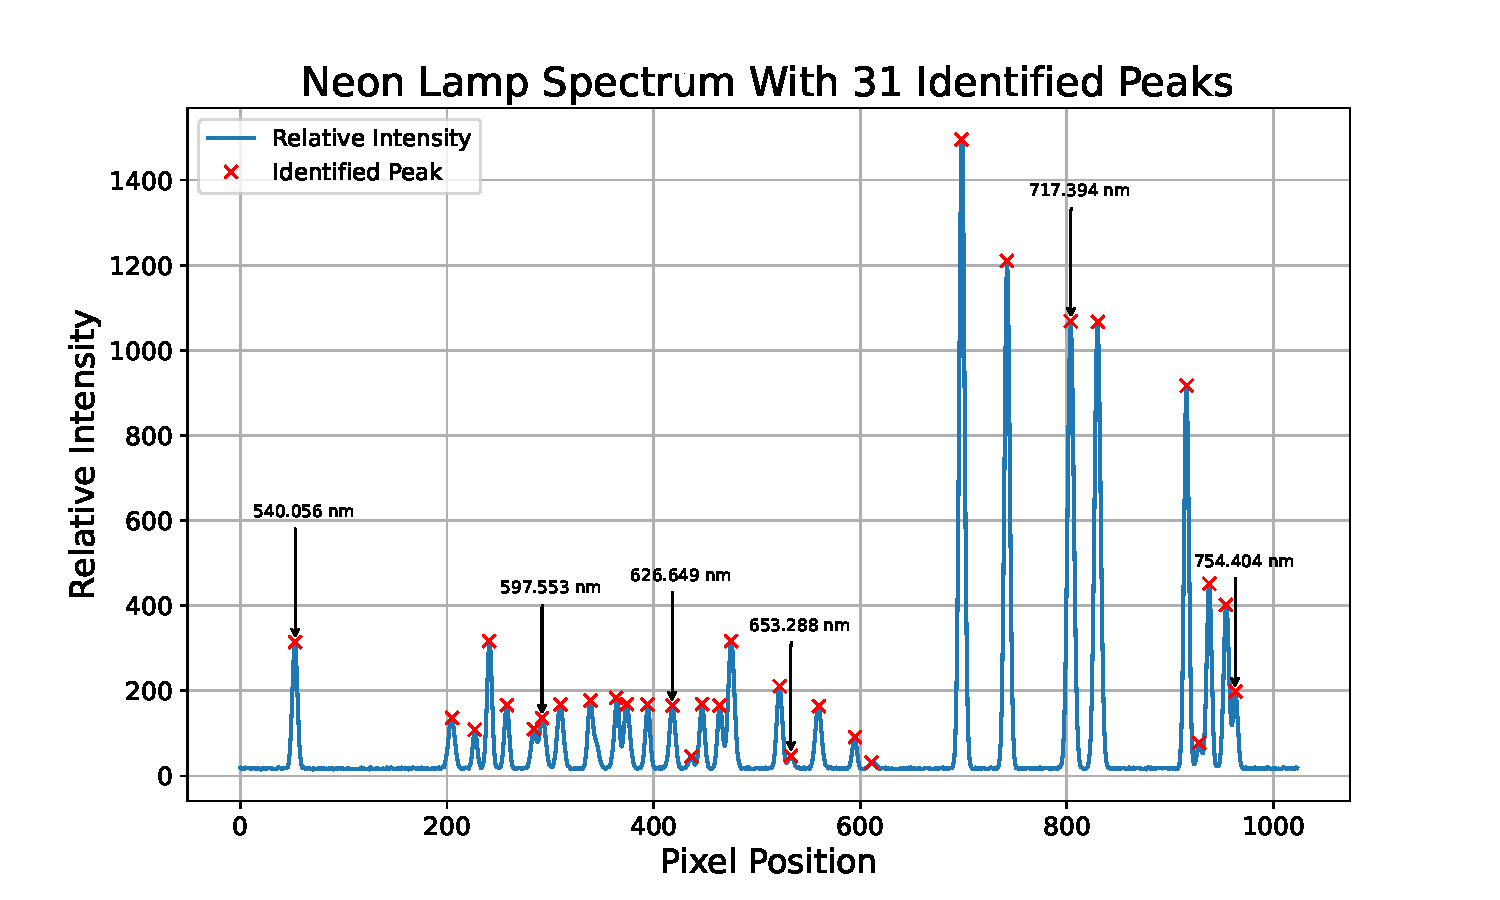
\includegraphics[width=.8\linewidth]{plots/neon_peaks.pdf}
  \caption{Identified peaks in the neon spectrum obtained using the USB4000 spectrometer that correspond to known wavelengths, every 6 peaks labelled to preserve clarity}
\end{figure}

\subsection{Shelyak Alpy Spectrometer}
\begin{figure}[H]
  \centering
  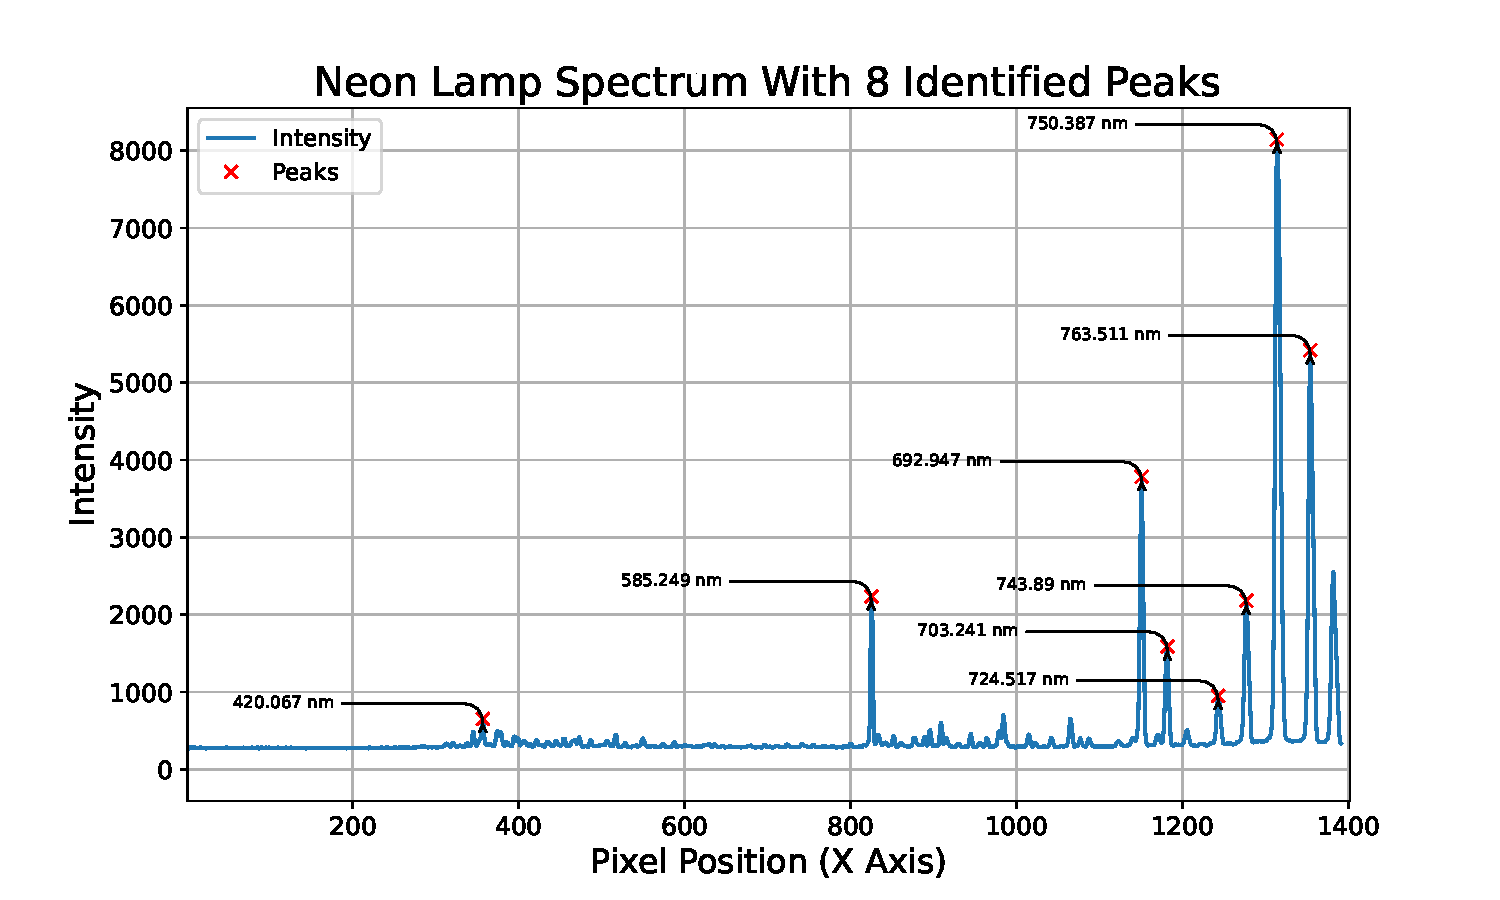
\includegraphics[width=.8\linewidth]{plots/obs_neon_peaks.pdf}
  \caption{Known peaks in the neon spectrum obtained using the Shelyak Alpy spectrograph that correspond to known wavelengths, all peaks labelled}
\end{figure}

\section{Additional Plots of Centroid Boundary Ranges}
\label{app:centroid_bounds}
\subsection{USB4000 Spectrometer}
\begin{figure}[H]
  \centering
  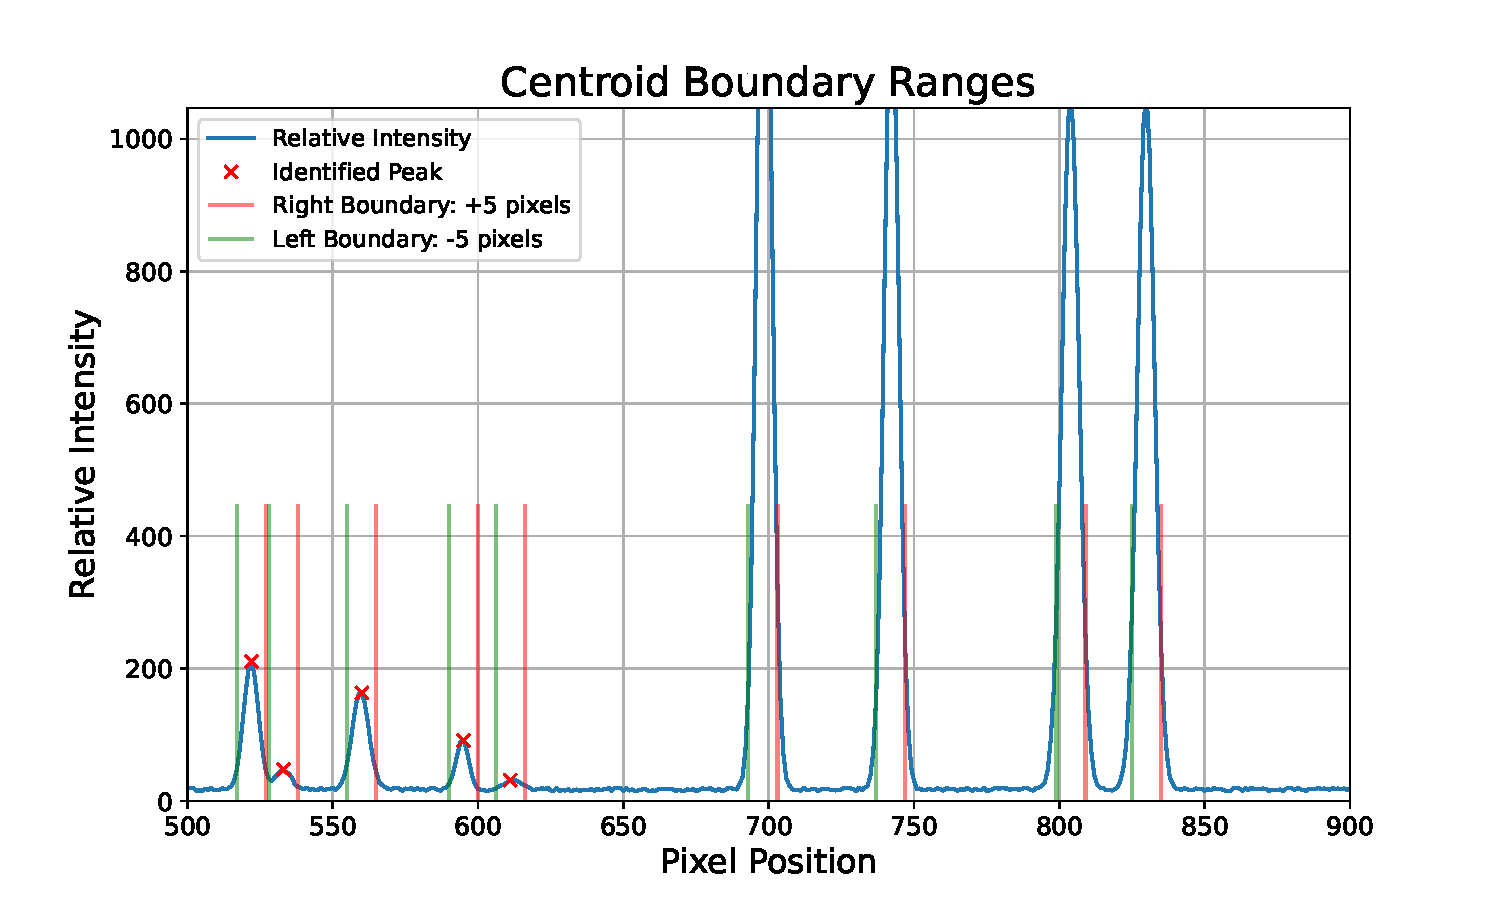
\includegraphics[width=.8\linewidth]{plots/neon_boundaries.pdf}
  \caption{Centroid boundary ranges for the USB4000 spectrometer}
\end{figure}
\subsection{Shelyak Alpy Spectrometer}
\begin{figure}[H]
  \centering
  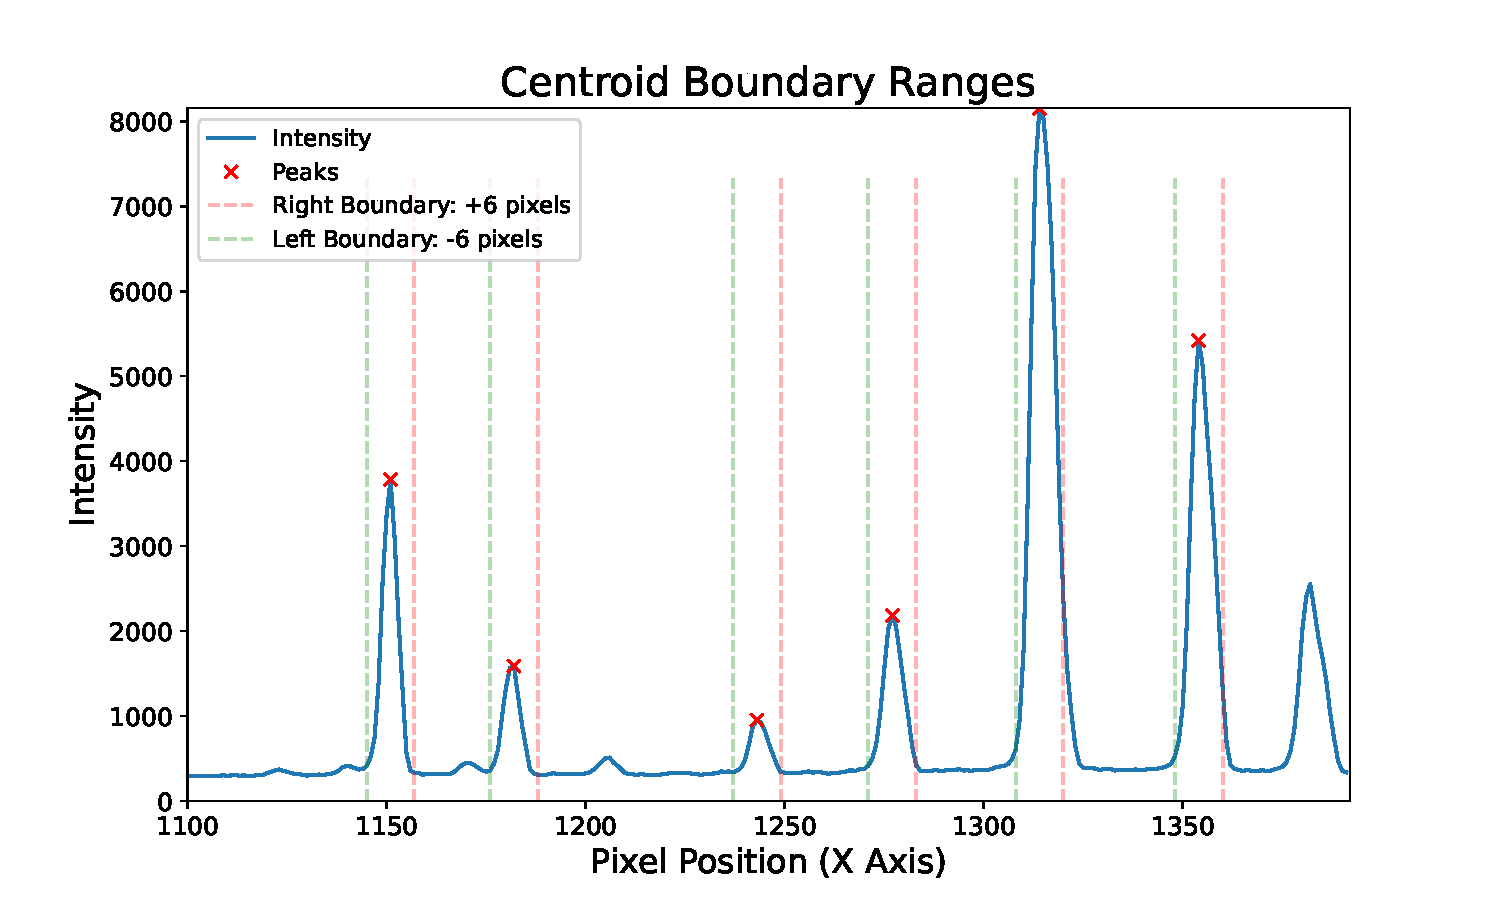
\includegraphics[width=.8\linewidth]{plots/obs_boundaries.pdf}
  \caption{Centroid boundary ranges for the Shelyak Alpy spectrograph}
\end{figure}

\section{Additional Centroid Plots}
\label{app:centroids}
\subsection{USB4000 Spectrometer}
\begin{figure}[H]
  \centering
  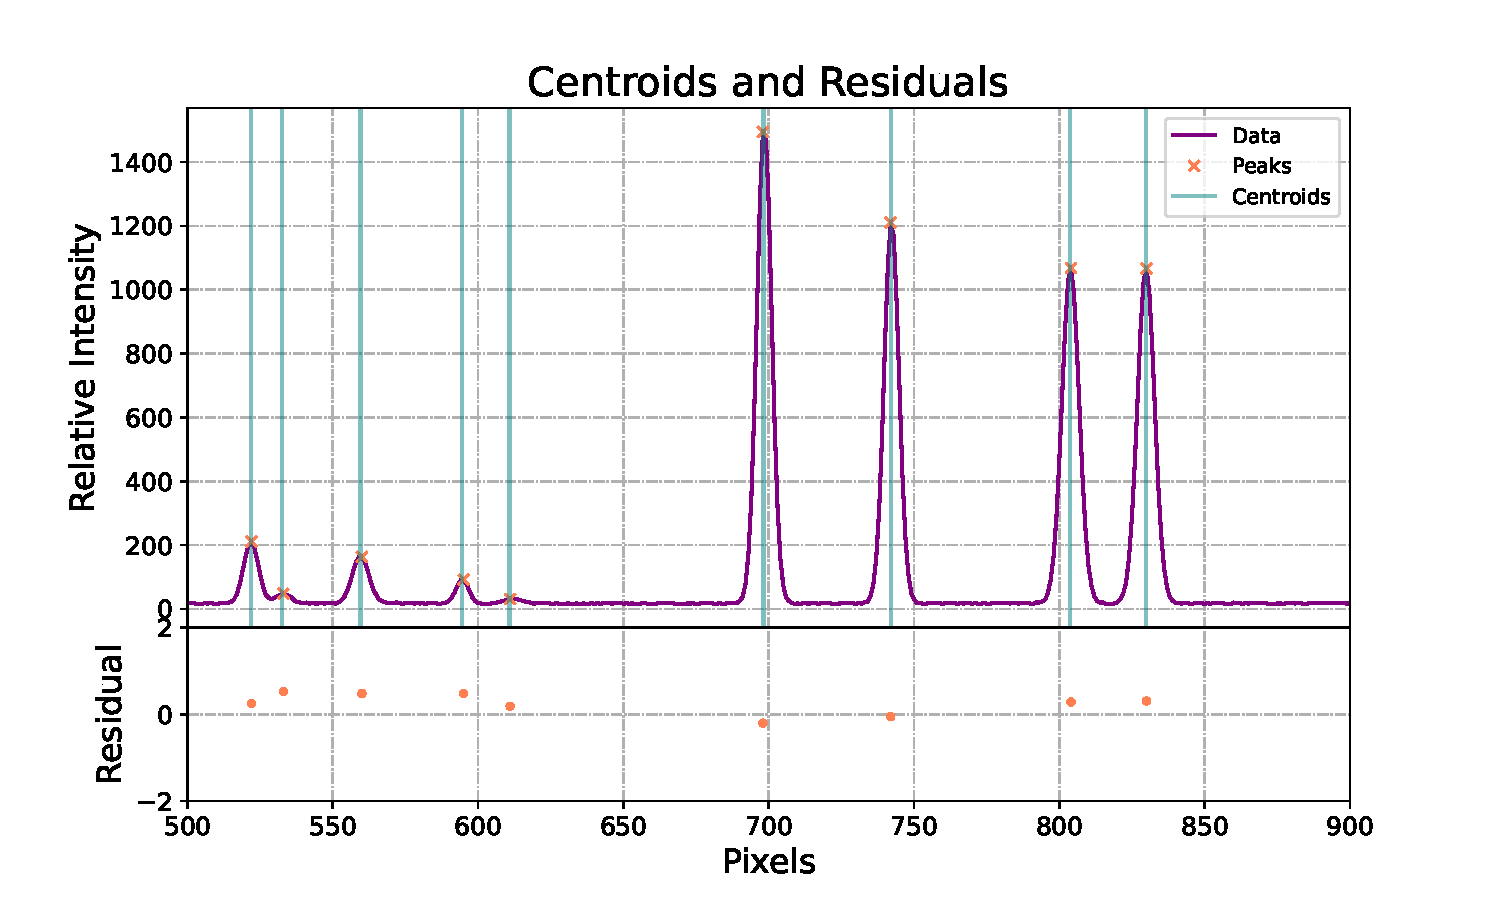
\includegraphics[width=.8\linewidth]{plots/neon_centroids.pdf}
  \caption{Centroids found for the USB4000 spectrometer}
\end{figure}

\subsection{Shelyak Alpy Spectrometer}
\begin{figure}[H]
  \centering
  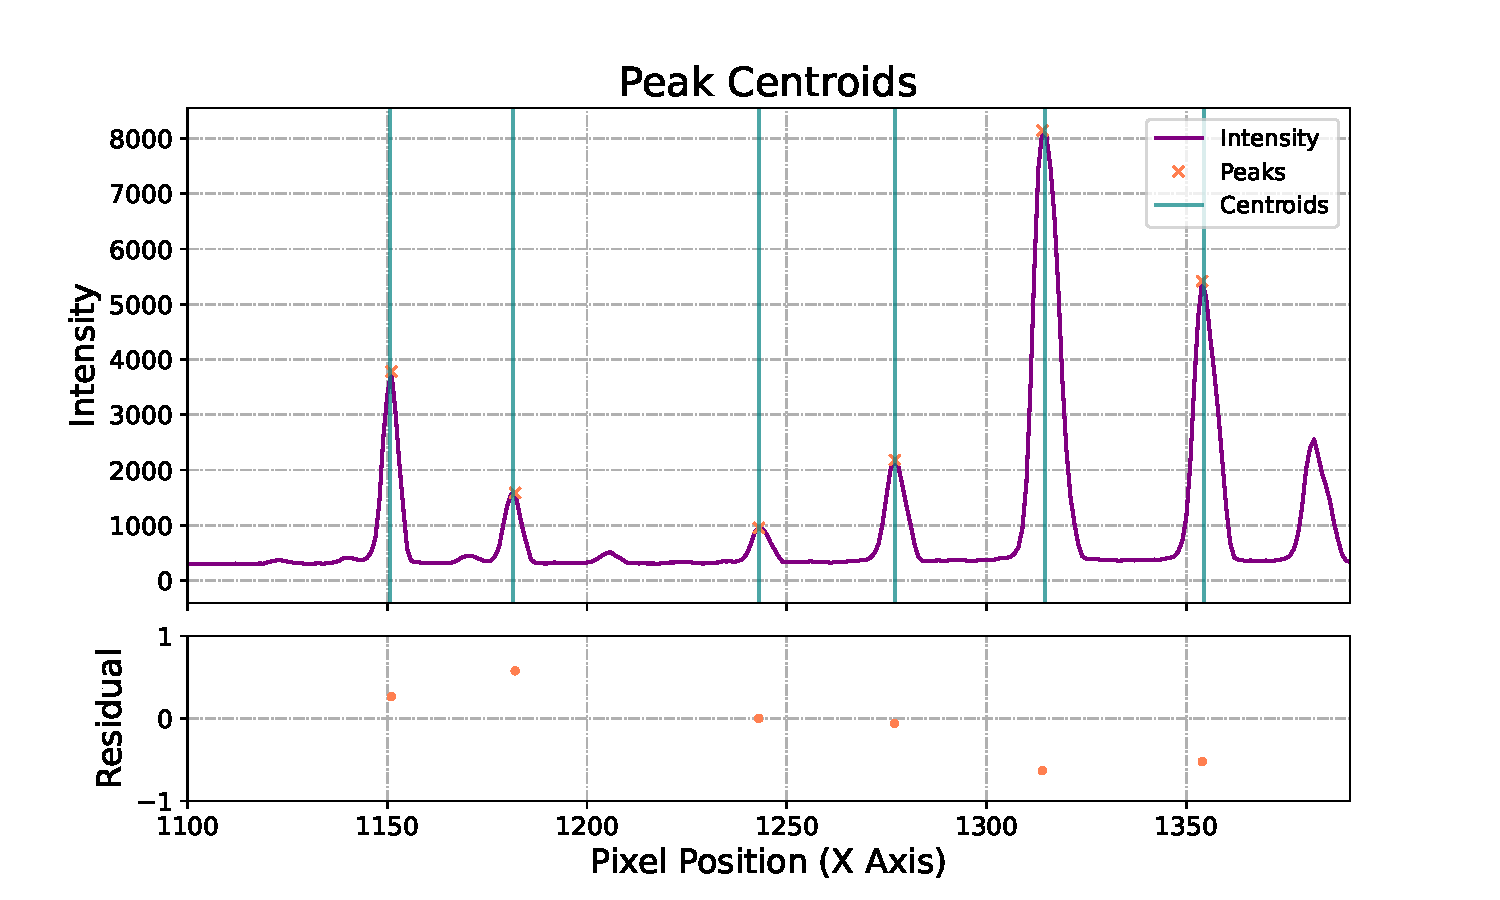
\includegraphics[width=.8\linewidth]{plots/obs_cen_residuals.pdf}
  \caption{Centroids calculated for the Shelyak Alpy spectrometer}
\end{figure}

\section{Additional Wavelength Solutions}
\label{app:solutions}
\subsection{USB4000 Spectrometer}

\begin{figure}[H]
  \centering
  \begin{subfigure}{.7\textwidth}
    \centering
    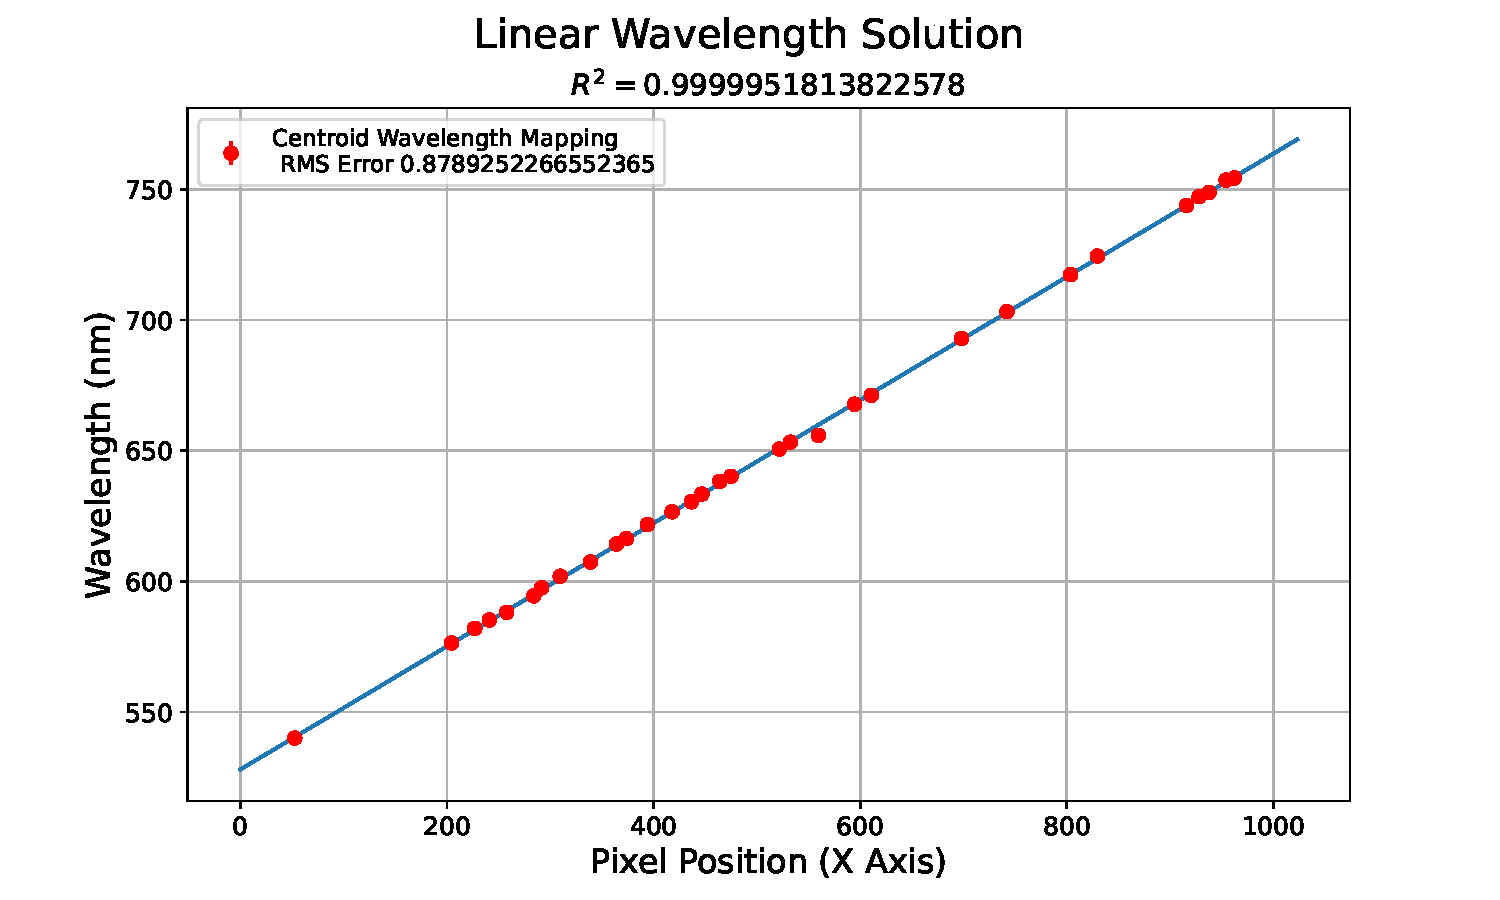
\includegraphics[width=\linewidth]{plots/neon_linear.pdf}
    \caption{Linear solution for the USB4000 spectrometer}
  \end{subfigure}%
  \begin{subfigure}{.3\textwidth}
    \centering
    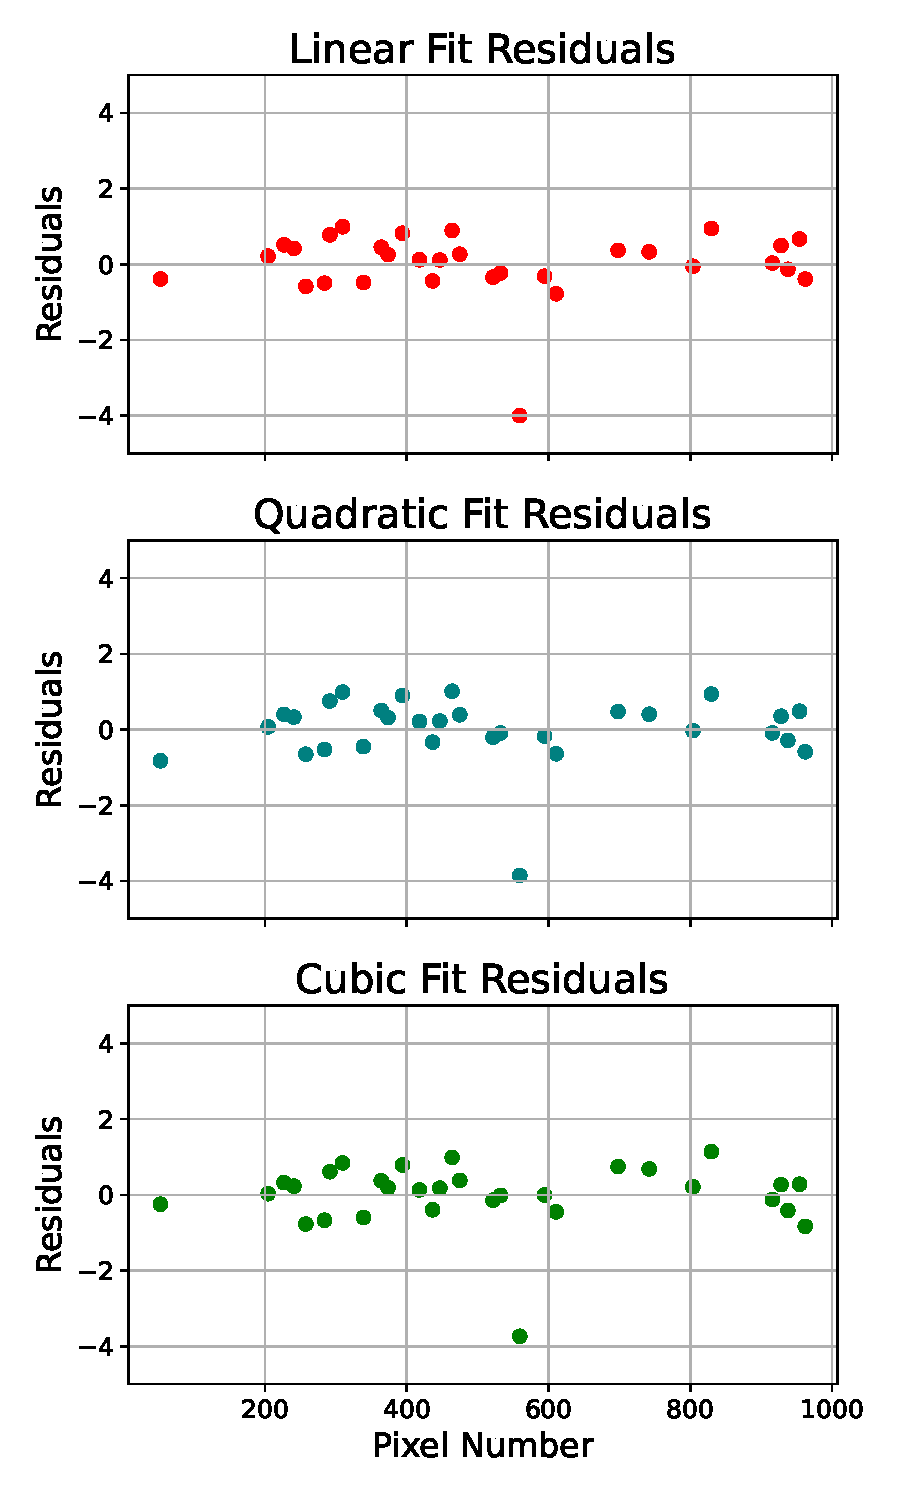
\includegraphics[width=\linewidth]{plots/neon_sol_residuals.pdf}
    \caption{Residuals for each polynomial degree.}
  \end{subfigure}
  \caption{Plot of the linear wavelength solution for the USB4000 spectrometer and the residuals}
\end{figure}

\begin{figure}[H]
  \centering
  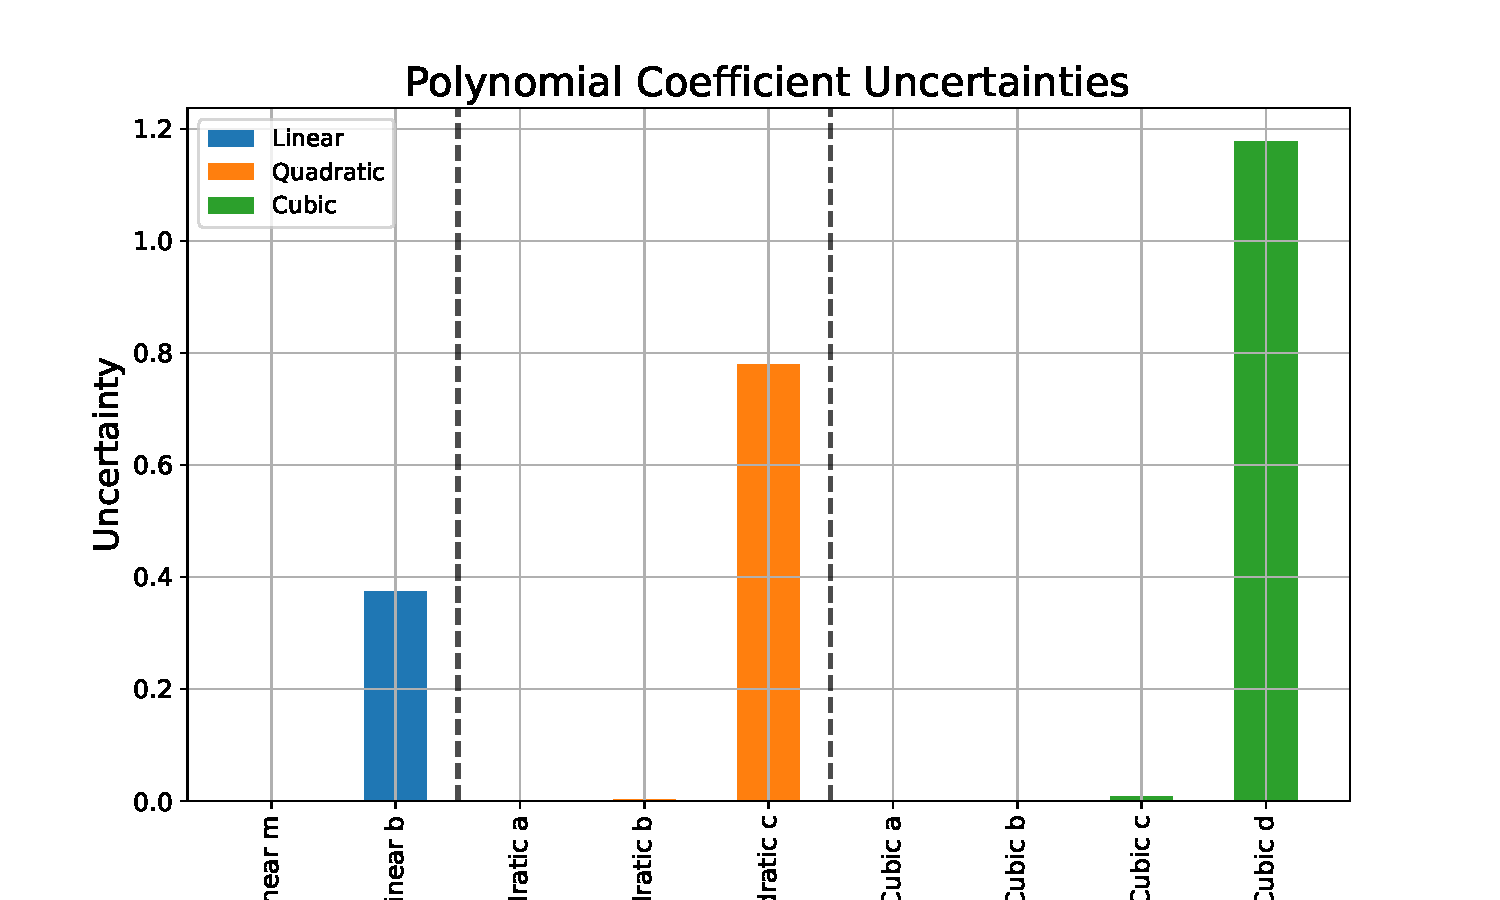
\includegraphics[width=.6\linewidth]{plots/neon_coef_uncertainty.pdf}
  \caption{Uncertainties of the coefficients for each solution for the USB4000 spectrometer, taken from the square root of the diagonals of the covariant matrix}
\end{figure}

\subsection{Shelyak Alpy Spectrometer}
\begin{figure}[H]
  \centering
  \begin{subfigure}{.7\textwidth}
    \centering
    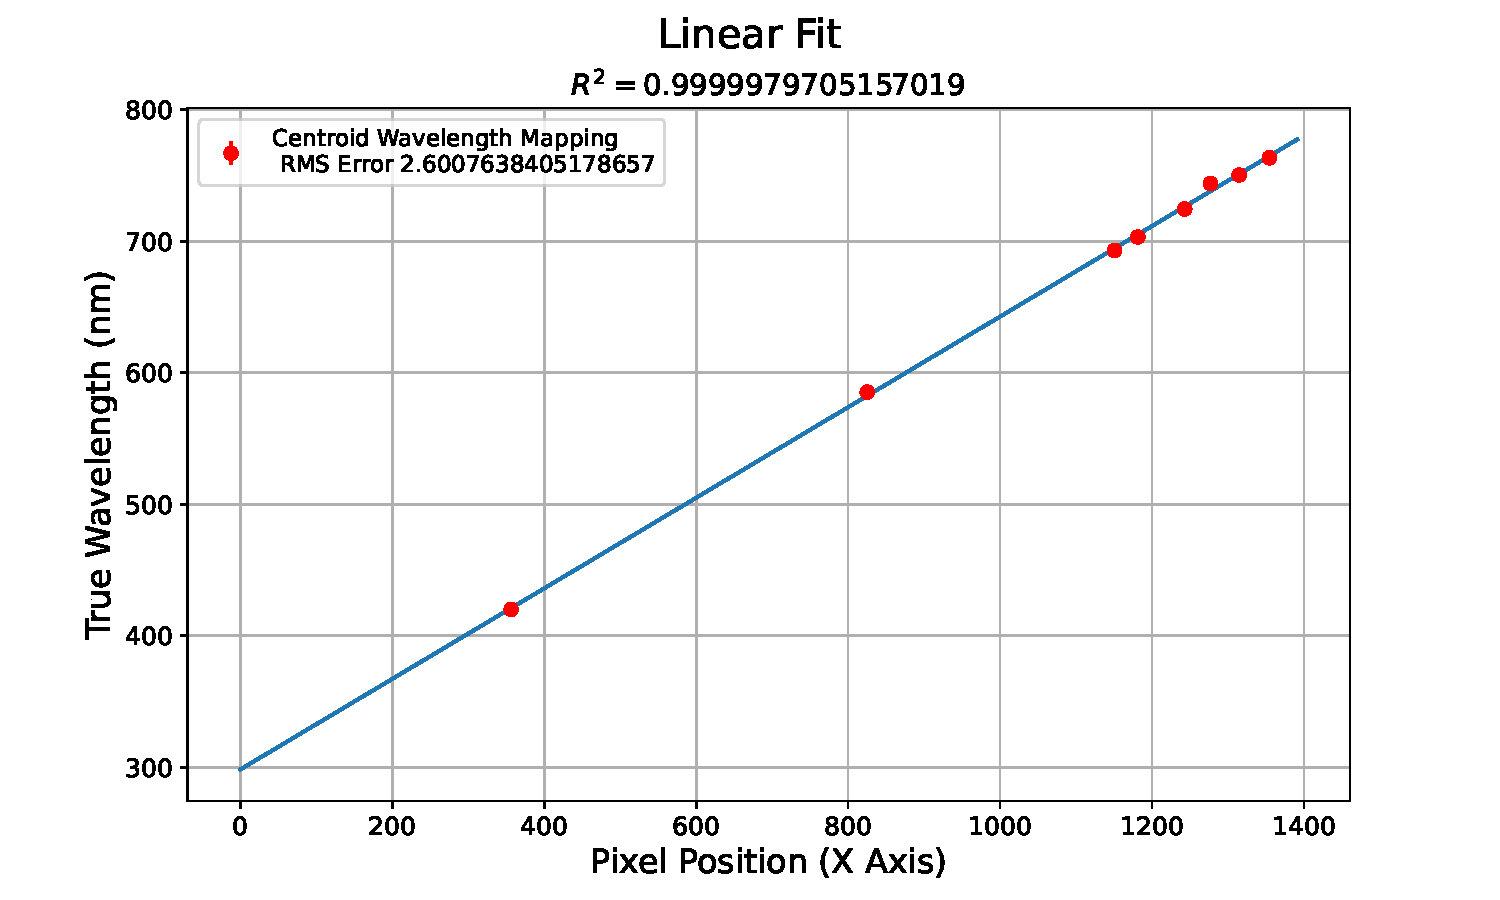
\includegraphics[width=\linewidth]{plots/obs_linear.pdf}
    \caption{Linear solution for the Shelyak Alpy spectrometer.}
  \end{subfigure}%
  \begin{subfigure}{.3\textwidth}
    \centering
    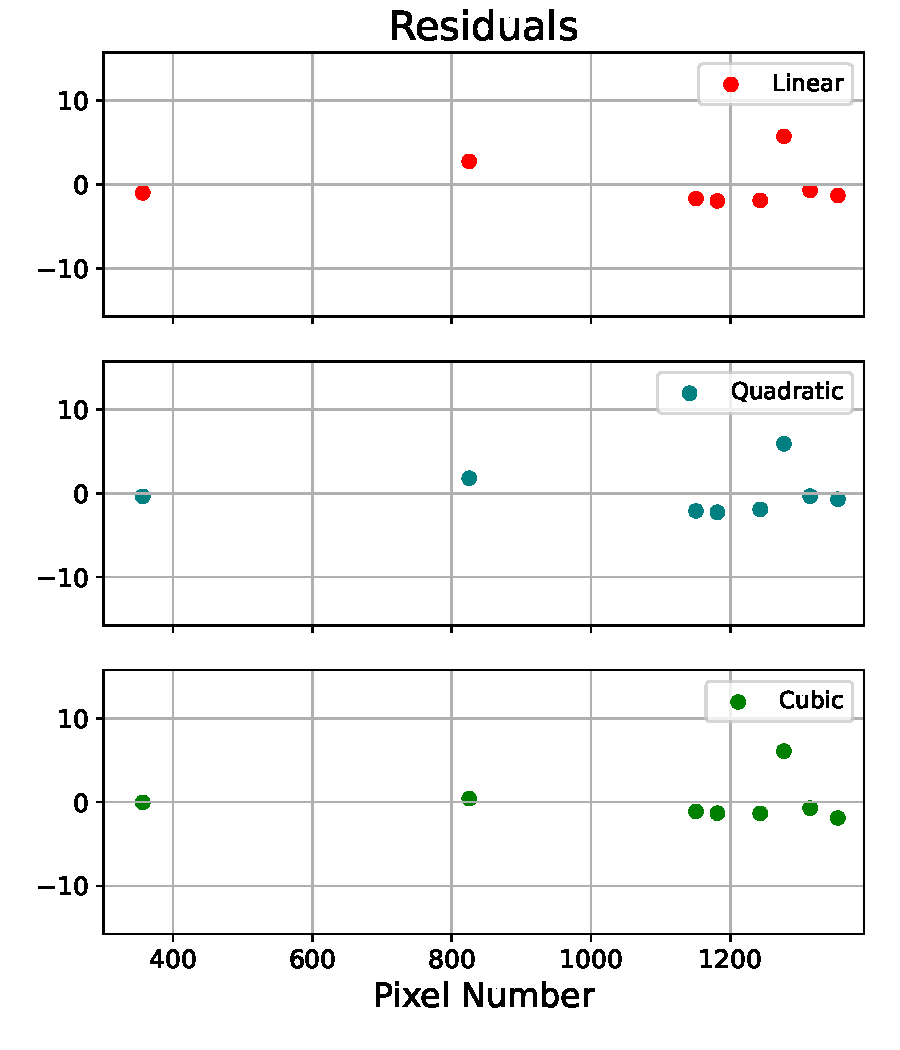
\includegraphics[width=\linewidth]{plots/obs_neon_residuals.pdf}
    \caption{Linear solution residuals.}
  \end{subfigure}
  \caption{Plot of the linear wavelength solution for the Shelyak Alpy spectrometer and the residuals}
\end{figure}

\begin{figure}[H]
\centering
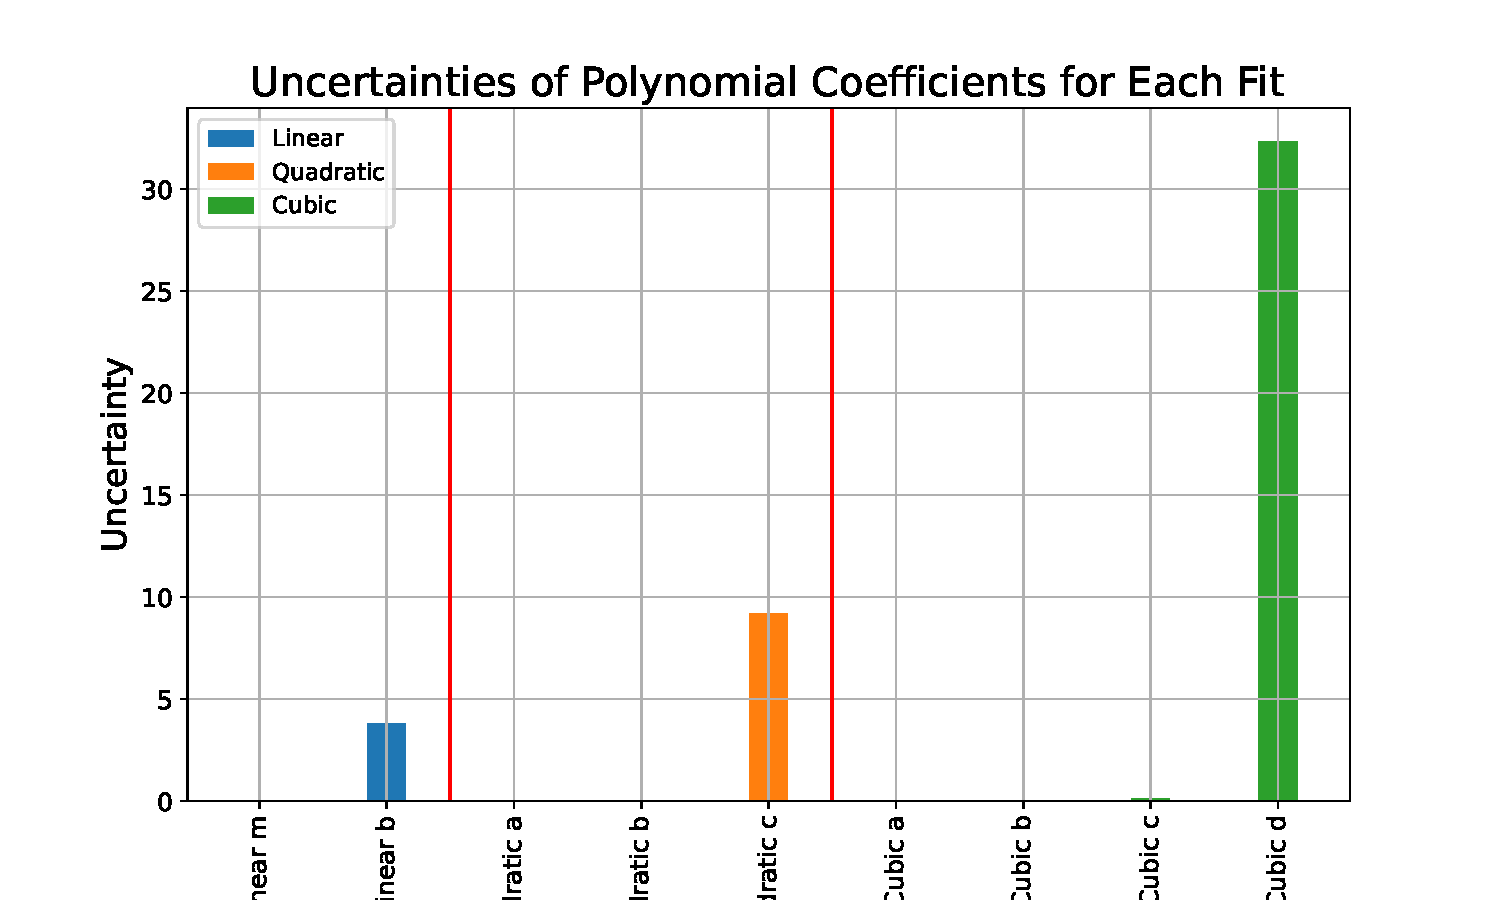
\includegraphics[width=.6\linewidth]{plots/obs_coef_uncertainty.pdf}
\caption{Uncertainties of the coefficients for each solution for the Shelyak Alpy Spectrometer, taken from the square root of the diagonals of the covariant matrix}
\label{fig:obs_coef}
\end{figure}

\section{Python Code}
\subsection{Python code for noise reduction in .fits files.}
\label{code:noise}
The following code, opens 1 science image, 3 darks and flats, and creates a median combined master dark and flat. It then applies 
the noise reduction techniques discussed in the report to export a final .fits file for further analysis. 
\begin{footnotesize}
\begin{verbatim}
from astropy.io import fits
import numpy as np

# Open Science file
science_file = fits.open("Part 3/GroupS/Moon_10S_20231026_21_50PM.fit")
science = np.array(science_file[0].data)

# Open Dark Files 
dark1 = fits.open("Part 3/GroupS/DARK_10S_20231026_21_58.fit")
dark2 = fits.open("Part 3/GroupS/DARK_10S_20231026_22_02.fit")
dark3 = fits.open("Part 3/GroupS/DARK_10S_20231026_22_03.fit")

# Open Flat Files 
flat1 = fits.open("Part 3/GroupS/Flat_5S_01.fit")
flat2 = fits.open("Part 3/GroupS/Flat_5S_02.fit")
flat3 = fits.open("Part 3/GroupS/Flat_5S_03.fit")

# Median Combine Flats
flat1_array = np.array(flat1[0].data)
flat2_array = np.array(flat2[0].data)
flat3_array = np.array(flat3[0].data)
flats_array = np.array([flat1_array,flat2_array,flat3_array])
master_flat = np.median(flats_array, axis=0)

# Median Combine Darks
dark1_array = np.array(dark1[0].data)
dark2_array = np.array(dark2[0].data)
dark3_array = np.array(dark3[0].data)
darks_array = np.array([dark1_array,dark2_array,dark3_array])
master_dark = np.median(darks_array, axis=0)

# My darks are all 10 second exposures, so assuming the noise scales linearly I 
# can just divide them by 2 for 5 seconds worth of noise 

master_dark_5S = master_dark / 2

# Steps
# 1. Subtract Master Dark From Science File which also includes Bias Noise 
science_sub_dark = science - master_dark_5S

# 2. Subtract dark from flat 
flat_sub_dark = master_flat - master_dark_5S

# 3. Divide 1 by 2
final_array  = science_sub_dark / flat_sub_dark

# Export processed FIT file 
final_fit = fits.PrimaryHDU(final_array)
final_fit.writeto('Part 3/GroupS/processed_fits/Moon_10S_Processed.fit')
\end{verbatim}
\end{footnotesize}
\subsection{Python code for peak finding and centroid placement}
\label{code:centroids}
The following code was used to find the peaks and centroids for the OH emission lines data set. The code for the 
other two data sets is identical, other than different height thresholds for the peaks and different range 
values for the centroid boundaries. 
\begin{footnotesize}
\begin{verbatim}
# Imports 
import numpy as np
from numpy import polyfit
from numpy import poly1d
from numpy import polyder
import scipy as sp
import scipy.constants as c
import matplotlib.pyplot as plt
import matplotlib.gridspec as gridspec

# Loading Projections Extracted Using DS9. Each sample has the exact same dimensions, 
# only shifted in the spatial direction.
projection = np.loadtxt("Lab 2/Part 2/ds9_2.dat")

known_lines = [16128.608,16194.615,16235.376,16317.161,16350.650
            ,16442.155,16502.365,16553.814]

# DS9 Y Pixel Ranges
ymin = 52
ymax = 217

f=11 # font size

pixels = np.arange(ymin,ymax)
emission_pixels = np.arange(ymin,ymax)
intensities = projection[:,1]

emission = np.loadtxt("Lab 2/Part 2/FE_2.dat")
emission_intensities = emission[:,1]

plt.rcParams["figure.figsize"] = (10,6)
plt.rcParams['font.size'] = 16
plt.rcParams['xtick.labelsize'] = 12
plt.rcParams['ytick.labelsize'] = 12

plt.title("Spectrum With Isolated OH Emission Lines")
plt.plot(pixels,intensities,color="teal", label="Intensity")
plt.xlabel("Pixel Position (Y Axis)")
plt.ylabel("Intensity")
plt.grid()
plt.legend(loc = 'best', fontsize = f)
plt.savefig("Lab 2/plots/OH_pixel_intensity.pdf")
plt.show()

# Peak Finding 
min_height = 0.1 * np.max(intensities)
initial_peaks, properties = sp.signal.find_peaks(intensities, height=min_height)
peaks = np.delete(initial_peaks,[0,6,8,9,11,13]) # Removing peaks that are not OH skylines
peaks = np.array(peaks)

# Peak Plotting
plt.rcParams["figure.figsize"] = (10,6)
plt.rcParams['font.size'] = 16
plt.rcParams['xtick.labelsize'] = 12
plt.rcParams['ytick.labelsize'] = 12

plt.title("{n} Identified Peaks".format(n=len(peaks)))
plt.xlabel("Pixel Position (Y Axis)")
plt.ylabel("Relative")
plt.plot(pixels,intensities,label="Intensity")
plt.plot(pixels[peaks],intensities[peaks], ls='', marker="x", color="red", label="Identified Peak")
for i, peak in enumerate(peaks):
if i % 2 == 0: # For every other peak labelled
  plt.annotate(str(known_lines[i])+" (A)", (pixels[peak], intensities[peak]), 
                xytext=(20,5), textcoords='offset points', 
                arrowprops=dict(facecolor='black', arrowstyle='->',connectionstyle="angle,angleA=0,angleB=90,rad=10"),
                label="Wavelengths (nm)", fontsize = f-3)
plt.grid(ls = '-')
plt.legend(loc = 'best', fontsize = f)
plt.savefig("Lab 2/plots/OH_Peaks.pdf")
plt.show()

# Finding Centroids
def centroid(x, I):
return np.sum(x*I)/np.sum(I)

# Determining Range Value For Centroids
range_value = 3
right_line_points = [pixels[peaks[i]]+range_value for i in range(len(peaks))]
left_line_points = [pixels[peaks[i]]-range_value for i in range(len(peaks))]

# Plotting Centroid Bounds
plt.title("Centroid Boundary Ranges")
plt.xlabel("Pixel Position (Y Axis)")
plt.ylim(0,np.max(intensities)+10)
plt.ylabel("Intensity")
plt.plot(pixels,intensities,label="Intensity")
plt.plot(pixels[peaks],intensities[peaks], ls='', marker="x", color="red", label="Peaks")
plt.vlines(right_line_points,color="red",ymin=0,ymax=.9*np.max(intensities),alpha=0.3, 
  linestyle="--", label="Right Boundary: +{p} pixels".format(p=range_value))
plt.vlines(left_line_points,color="green",ymin=0,ymax=.9*np.max(intensities),alpha=0.3, 
  linestyle="--", label="Left Boundary: -{p} pixels".format(p=range_value))
plt.legend(loc = 'best', fontsize = f)
plt.grid(".-")
plt.savefig("Lab 2/plots/OH_Centroid_Boundaries.pdf")
plt.show()

# Calculate Centroids
centroids = [centroid(pixels[peaks[i]-range_value:peaks[i]+range_value], 
  intensities[peaks[i]-range_value:peaks[i]+range_value]) for i in range(len(peaks))]
centroid_residuals = np.array(centroids) - np.array(pixels[peaks])

# root mean square error for centroids
rmse_centroid = np.sqrt(np.mean(centroid_residuals**2))
print("Centroid RMS Error: {r}".format(r=rmse_centroid))

# Plotting The Centroids and Residuals
fig = plt.figure(figsize=(10,6))
gs = gridspec.GridSpec(2, 1, height_ratios=[3, 1], hspace = 0.1)
ax0 = plt.subplot(gs[0])
ax0.set_title("Centroid Pixel Positions")
ax1 = plt.subplot(gs[1], sharex = ax0)
ax1.set_ylim(-0.5,0.5)
ax0.plot(pixels, intensities, color = 'purple', label = 'Intensity')
ax0.plot(pixels[peaks], intensities[peaks], color = 'coral', ls = '', marker = 'x',
      ms = 5, label = 'Peaks')
[ax0.axvline(c, color = 'teal', alpha = 0.7, label = 'Centroids') if c == centroids[0]
else ax0.axvline(c, color = 'teal', alpha = 0.7) for c in centroids]
ax1.plot(pixels[peaks], pixels[peaks] - centroids, ls = '', marker = '.', color = 'coral')
ax1.set_xlabel('Pixel Position (Y Axis)')
ax0.set_ylabel('Intensity')
ax1.set_ylabel('Residual')
plt.setp(ax0.get_xticklabels(), visible = False)
ax0.legend(loc = 'best', fontsize = f)
ax0.grid(ls = '-.')
ax1.grid(ls = '-.')
plt.savefig("Lab 2/plots/OH_Centroids_Residuals.pdf")
plt.show()


\end{verbatim}
\end{footnotesize}
\subsection{Python code for finding wavelength solutions and plotting them}
This code was used on the OH emission data set. The code for the other two are almost identical except with a few variable names changed and plot titles. 
\begin{footnotesize}
\begin{verbatim}
# Imports 
import numpy as np
from numpy import polyfit
from numpy import poly1d
from numpy import polyder
import scipy as sp
import scipy.constants as c
import matplotlib.pyplot as plt
import matplotlib.gridspec as gridspec

# Wavelengths picked out by hand
known_lines = [16128.608,16194.615,16235.376,16317.161,16350.650
,16442.155,16502.365,16553.814]


# Finding the fits 
linear_fit, linear_cov = polyfit(centroids,known_lines,1,full=False, cov=True)
lin = poly1d(linear_fit)
quadratic_fit, quad_cov = polyfit(centroids,known_lines,2,full=False, cov=True)
quad = poly1d(quadratic_fit)
cubic_fit, cub_cov = polyfit(centroids,known_lines,3,full=False, cov=True)
cub=poly1d(cubic_fit)

# Calculating Fit for all pixels
linear_values_all = lin(pixels)
quad_values_all = quad(pixels)
cub_values_all = cub(pixels)

# Calculating fit only for centroid point
linear_values_cen = lin(centroids)
quad_values_cen = quad(centroids)
cub_values_cen = cub(centroids)

values=[linear_values_all,quad_values_all,cub_values_all]

# Calculate Residuals
linear_residuals = np.array(known_lines) - np.array(linear_values_cen)
quad_residuals = np.array(known_lines) - np.array(quad_values_cen)
cub_residuals = np.array(known_lines) - np.array(cub_values_cen)
residuals=[linear_residuals,quad_residuals,cub_residuals]

# root mean square for residuals
rmse = []
for res in residuals:
  rmse.append(np.sqrt(np.mean(res**2)))

# Calculate Uncertainty of Fit For Coefficients
linear_uncertainty = np.sqrt(np.diag(linear_cov))
quad_uncertainty = np.sqrt(np.diag(quad_cov))
cub_uncertainty = np.sqrt(np.diag(cub_cov))
uncertainty_coefficients = [linear_uncertainty,quad_uncertainty,cub_uncertainty]
print("Uncertainty of Coefficients")
print("----------")
for u in uncertainty_coefficients:
  print(u)

linear_coef_names = ['m', 'b']
quad_coef_names = ['a', 'b', 'c']
cub_coef_names = ['a', 'b', 'c', 'd']
coef_names = [linear_coef_names, quad_coef_names, cub_coef_names]
fit_names = ['Linear', 'Quadratic', 'Cubic']
fig, ax = plt.subplots()
current_x = 0
for i, uncertainty in enumerate(uncertainty_coefficients):
  x_values = [f"{fit_names[i]} {coef_names[i][j]}" for j in range(len(uncertainty))]
  ax.bar(x_values, uncertainty, width=0.5, align="center", label="{f}".format(f=fit_names[i]))
  current_x += len(uncertainty)
  if i < len(uncertainty_coefficients) - 1:
    ax.axvline(current_x - 0.5, color='black', alpha=0.7, linestyle='--', linewidth=2)
ax.set_xlabel('Fit')
ax.set_ylabel('Uncertainty')
ax.set_title('Coefficient Uncertainties for Each Fit')
plt.xticks(rotation=90)
plt.grid(".-")
plt.legend(loc='best', fontsize=f)
plt.savefig("Lab 2/plots/OH_Coef_Uncerctainty.pdf")
plt.show()

# R^2 Values
print("----------")
print("R^2 Values")
print("----------")
r_array = []
for val in range(0,len(values)):
  total_square_sum = np.sum((values[val] - np.mean(values[val]))**2)  # total sum of squares
  res_square_sum = np.sum(residuals[val]**2)  # residual sum of squares
  r_squared = 1 - (res_square_sum / total_square_sum)  # R^2 value
  print("R^2 = {r}".format(r=r_squared))
  r_array.append(r_squared)

plt.suptitle("Linear Wavelength Solution")
plt.title("$R^2 = ${r}".format(r=r_array[0]),fontsize=f+3)
plt.errorbar(centroids, known_lines, yerr=rmse[0], fmt='o', 
  label="Centroid Wavelength Mapping \n RMS Error {r}".format(r=rmse[0]), color="red")
plt.plot(pixels,lin(pixels))
plt.xlabel("Pixel Position (Y Axis)")
plt.ylabel("True Wavelength (Angstroms)")
plt.grid(".-")
plt.legend(loc = 'best', fontsize = f)
plt.savefig("Lab 2/plots/OH_Linear.pdf")
plt.show()

plt.suptitle("Quadratic Wavelength Solution")
plt.title("$R^2 = ${r}".format(r=r_array[1]),fontsize=f+3)
plt.errorbar(centroids, known_lines, yerr=rmse[1], fmt='o', 
  label="Centroid Wavelength Mapping \n RMS Error {r}".format(r=rmse[1]), color="red")
plt.plot(pixels,quad(pixels))
plt.xlabel("Pixel Position (Y Axis)")
plt.ylabel("True Wavelength (A)")
plt.grid(".-")
plt.legend(loc = 'best', fontsize = f)
plt.savefig("Lab 2/plots/OH_Quadratic.pdf")
plt.show()

plt.suptitle("Cubic Wavelength Solution")
plt.title("$R^2 = ${r}".format(r=r_array[2]),fontsize=f+3)
plt.errorbar(centroids, known_lines, yerr=rmse[2], fmt='o', 
  label="Centroid Wavelength Mapping \n RMS Error {r}".format(r=rmse[2]), color="red")
plt.plot(pixels,cub(pixels))
plt.xlabel("Pixel Position (Y Axis)")
plt.ylabel("True Wavelength (A)")
plt.grid(".-")
plt.legend(loc = 'best', fontsize = f)
plt.savefig("Lab 2/plots/OH_Cubic.pdf")
plt.show()

# All fits plotted and extended to check for overfititng
pixels_extended = np.arange(ymin-len(pixels),ymax+len(pixels))
plt.title("Wavelength Solutions Compared")
plt.plot(pixels_extended,lin(pixels_extended), color="orange", 
  label="Linear: RMS Error {r}".format(r=np.round(rmse[0],2)) ,alpha=0.5, ls="--")
plt.plot(pixels_extended,quad(pixels_extended), color="blue", 
  label="Quadratic: RMS Error {r}".format(r=np.round(rmse[1],2)), alpha=0.5, ls="--")
plt.plot(pixels_extended,cub(pixels_extended), color="green", 
  label="Cubic: RMS Error {r}".format(r=np.round(rmse[2],2)), alpha=0.5, ls="--")
plt.scatter(centroids,known_lines, color="red", label="Centroid Wavelength Mapping")
plt.xlabel("Pixel Position (Y Axis)")
plt.ylabel("True Wavelength")
plt.grid(".-")
plt.legend(loc="best",fontsize=f)
plt.savefig("Lab 2/plots/OH_Sol_Comparison.pdf")
plt.show()

# Plot Residuals
bound = np.max(linear_residuals) + 10
fig, ax = plt.subplots(3, 1, figsize=(6, 7), sharex=True)
ax[0].scatter(centroids, residuals[0], color="red",label="Linear")
ax[0].set_title("Residuals")
ax[0].set_ylim(-bound,bound)
ax[0].set_xlim(ymin,ymax)
ax[0].grid(True)
ax[0].legend(loc = 'best', fontsize = f)
ax[1].scatter(centroids, residuals[1], color="teal", label="Quadratic")
ax[1].set_ylim(-bound,bound)
ax[1].set_xlim(ymin,ymax)
ax[1].legend(loc = 'best', fontsize = f)
ax[1].grid(True)
ax[2].scatter(centroids, residuals[2], color="green", label="Cubic")
ax[2].set_xlabel("Pixel Number")
ax[2].set_xlim(ymin,ymax)
ax[2].set_ylim(-bound,bound)
ax[2].legend(loc = 'best', fontsize = f)
ax[2].grid(True)
plt.tight_layout()
plt.subplots_adjust(top=0.95)  
plt.savefig("Lab 2/plots/OH_Sol_Residuals.pdf")
plt.show()
\end{verbatim}
\end{footnotesize}
\label{code:solution}
\subsection{Python code for calculating temperature using Wien's Law}
\begin{footnotesize}
\begin{verbatim}
# Imports 
import numpy as np
from numpy import polyfit
from numpy import poly1d
from numpy import polyder
import scipy as sp
import scipy.constants as c
import matplotlib.pyplot as plt
import matplotlib.gridspec as gridspec

# Finding Peak Intensity Wavelength 
max_wavelength = linear_values_all[np.argmax(bb_data)]
print("Wavelength of Highest Intensity is : {w}nm".format(w=max_wavelength))

# Now using Wien's displacement law to find temperature
wavelength_bb_meters = max_wavelength * 10**(-9)
print("Temperature of blackbody is: {t} Kelvin".format(t = c.Wien / wavelength_bb_meters))
\end{verbatim}
\end{footnotesize}
\label{code:temperature}
\subsection{Python code for calculating velocity using Doppler shift.}
\begin{footnotesize}
\begin{verbatim}
# Imports 
import numpy as np
from numpy import polyfit
from numpy import poly1d
from numpy import polyder
import scipy as sp
import scipy.constants as c
import matplotlib.pyplot as plt
import matplotlib.gridspec as gridspec

# Calculating Velocity of Emission Using Doppler Shift Formula

intrensic_wavelength = 1.6439981 # microns
intrensic_wavelength_angstroms = intrensic_wavelength*1e4 # angstroms
velocity = c.c * (observed_wavelength-intrensic_wavelength_angstroms)/intrensic_wavelength_angstroms
print("Velocity of FE2 Emission is {v} km/s".format(v=velocity*1e-3))
\end{verbatim}
\end{footnotesize}


\label{code:velocity}
\subsection{Python code for error propagation}
\label{code:error}
This code was used to calculate the error for the OH emission lines data set, using the three sources of error discussed in the report. 
\begin{footnotesize}
  \begin{verbatim}

# Imports 
import numpy as np
from numpy import polyfit
from numpy import poly1d
from numpy import polyder
import scipy as sp
import scipy.constants as c
import matplotlib.pyplot as plt
import matplotlib.gridspec as gridspec

# Error Propogation 
# Sources of error are initial centroid placement, polynomial fitting, and peak wavelength centroid placement

# df/dx for the two centroid placements were found by running the program many times and finding 
# the rate of change of the velocity per unit pixel. 

derivative = polyder(quad)
peak_derivative = derivative(peak_centroid[0])
propogated_error = np.sqrt((44.15)**2*rmse_centroid+(peak_derivative)**2*rmse[1]+(43.81)**2*rmse_peak)
print("Propogated Error is {p} km/s".format(p=propogated_error))

  \end{verbatim}
\end{footnotesize}


\end{appendices}

\end{document}
